\documentclass[12pt]{article}

\usepackage{aircrafts}
\title{\Large Energy Analysis of Controlled ODE Models\\ with Mass Variation}
\newcommand{\authorinfo}{Faculty of Mathematics and Computer Science; e-mail: \texttt{2511001864@student.hcmus.edu.vn}}
\author{
  \normalsize Pham Ngoc Gia Bao\\
  \normalsize University of Science, VNU-HCM\footnote{\authorinfo}
}
\date{\normalsize\today}

\makeatletter
\renewcommand{\@maketitle}{%
  \newpage
  \vspace*{-2cm}%
  \begin{center}%
  \let \footnote \thanks
    {\LARGE \@title \par}%
    \vskip 1.5em%
    {\large
      \lineskip .5em%
      \begin{tabular}[t]{c}%
        \@author
      \end{tabular}\par}%
    \vskip 1em%
    {\large \@date}%
  \end{center}%
  \par
  \vskip 1.5em}
\makeatother

\begin{document}

\maketitle
\begin{abstract}
In this expository note, we study simplified controlled ODE models for 1D motion with gravity, drag, feedback control, and mass variation. 
We analyze the resulting closed-loop error equations through characteristic roots and energy methods. 
The same framework is then extended to aircraft mass-dependent damping and spacecraft propulsion.
\end{abstract}
\tableofcontents

\section*{Introduction}
In classical mechanics, Newton's second law gives a fundamental relation between force, mass, velocity, and acceleration~\cite{arnold_classical_mechanics}. For a body with constant mass, this relation can be written as
\[
 F = ma = m\dot v = m\ddot h.
\]
To simplify the setting, we impose several assumptions. All motions considered in this note are 1D. In Part I, the moving body is assumed to have constant mass.  The environment contains gravity, and the drag force is assumed to be linear in velocity. Moreover, aerodynamic details, rotation, thrust direction, and turbulence are ignored. The purpose of these assumptions is to isolate a basic ODE model and study the mechanism of motion and stability in a controlled system.

We choose a 1D coordinate system whose positive direction is upward. Suppose that the height of the body at time $t$ is $h(t)$, and suppose that we want the body to approach a desired height $h_d$, which is treated as a constant. By Newton's second law, the motion can be written in the form
\[
 h'(t) = v(t),\quad v'(t) = u(t) - g - cv(t).
\]
The first equation states that velocity is the derivative of height, while the second equation says that the acceleration is increased by the control input and reduced by gravity and linear drag. We define the tracking error by
\[
 e(t) = h(t) - h_d.
\]
Thus, the stabilization problem becomes the question of whether $e(t)$ tends to zero as time evolves. We choose the control input according to the feedback law
\[
 u(t) = g - k_1e(t) - k_2v(t),
\]
where $k_1$ and $k_2$ are constants to be chosen. This feedback law means that the control input is adjusted according to the current tracking error and velocity. Substituting this law into the motion equation gives the CLE (Closed-Loop Error) equation
\[
 e'' + (k_2 + c)e' + k_1e = 0.
\]
This is a second-order linear ODE, and the main part of this project is organized around this equation. The central question is how the control input, through the feedback parameters, affects stability and damping behavior.

The note is organized around three themes: the derivation and stability of the CLE equation, its energy and variational structure, and its extension to mass-dependent aircraft and spacecraft models.
For aircraft motion, fuel burn makes the normalized drag coefficient time-dependent, leading to a CLE equation with variable damping. 
A modified Lyapunov energy is then used to prove convergence of the aircraft error dynamics. 
For spacecraft motion, propellant loss is also the mechanism that generates thrust. 
This gives the ideal rocket equation and an energy-based criterion for planetary escape.

All source files, numerical scripts, and the revision history of this report
are available at \url{https://github.com/aleksis-arendt/aircrafts}.
\part{Controlled ODE Model and Energy Analysis}
\section{1D Motion Model}

\subsection{Construction}
The notation used in the 1D model is summarized in Table~\ref{tab:1d-notation}.

We choose the vertical coordinate so that the positive direction is upward. Let $m$ denote the mass of the moving body. In the basic model, $m$ is assumed to be constant, $g$ is treated as a constant gravitational acceleration, and the desired height $h_d$ is fixed. The drag force is modeled as a linear function of velocity, namely

\[
 F_{\mathrm{drag}} = -bv.
\]
For simplicity, we ignore nonlinear drag, lift, rotation, thrust-direction constraints, turbulence, and mass variation.

The forces acting on the body are the thrust force $T(t)$, the gravitational force $-mg$, and the linear drag force $-bv(t)$. By Newton's second law, for a body with constant mass, the net force equals mass times acceleration~\cite{arnold_classical_mechanics}. Hence
\[
 m h''(t) = T(t) - mg - bv(t).
\]
Since $v(t) = h'(t)$, this can be written as
\begin{equation}\label{eq:newton-motion}
 T(t) - mg - bh'(t) = m h''(t).
\end{equation}

\begin{figure}[h]
\centering
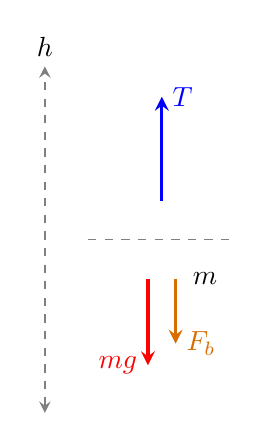
\begin{tikzpicture}[scale=1.1,>=stealth]
    \draw[<->,thick,dashed,gray] (-1.35,-2.0) -- (-1.35,2)
        node[above,black] {$h$};
    \draw[dashed,gray] (-0.85,0) -- (0.85,0);
    \node[scale=2.6,rotate=90] at (0,0) {\Plane};
    \node at (0.5,-0.45) {$m$};

    \draw[->,very thick,blue] (0,0.45) -- (0,1.65)
        node[right,blue] {$T$};
    \draw[->,very thick,red] (-0.16,-0.45) -- (-0.16,-1.45)
        node[left,red] {$mg$};
    \draw[->,very thick,orange!85!black] (0.16,-0.45) -- (0.16,-1.2)
        node[right,orange!85!black] {$F_b$};

\end{tikzpicture}
\caption{Forces in the vertical model.}
\end{figure}
Define the normalized control input and drag coefficient by
$u(t) = \frac{T(t)}{m},$ and $c = \frac{b}{m}.$
Here $u(t)$ has unit $\mathrm{m/s^2}$, while $c$ has unit $\mathrm{s^{-1}}$. Dividing \eqref{eq:newton-motion} by $m$ gives
\begin{equation}\label{eq:normalized-motion}
 h''(t) = u(t) - g - cv(t).
\end{equation}
Equivalently, using $v(t) = h'(t)$, the 1D motion model becomes
\begin{equation}\label{eq:motion-system}
\boxed{
\begin{cases}
 h'(t) = v(t),\\
 v'(t) = u(t) - g - cv(t).
\end{cases}
}
\end{equation}

The constant $c = b/m$ is the normalized linear drag coefficient. The term $-cv(t)$ represents the acceleration-level effect of linear drag. 
Since this term has the opposite sign of the velocity, it always acts against the direction of motion. 

For example, if $v(t) > 0$, then the body is moving upward and $-cv(t) < 0$, so drag reduces the upward acceleration. 
If $v(t) < 0$, then the body is moving downward and $-cv(t) > 0$, so drag acts upward and slows the downward motion. 
In this sense, $c$ measures the strength of the physical damping caused by the surrounding medium.

After this normalization, every term in the second equation has the unit of acceleration, $\mathrm{m/s^2}$. The term $u(t)$ represents the upward control acceleration, while $-g$ and $-cv(t)$ represent the effects of gravity and linear drag.
\subsection{Tracking Error and Feedback Law}
Let $h_d$ be the desired height. The goal is to design a feedback law for the control input $u(t)$ such that the height $h(t)$ approaches $h_d$ as time evolves. To measure the deviation between the current height and the desired height, we introduce the \textit{tracking error} $e(t) = h(t) - h_d.$ Thus, the stabilization problem becomes the problem of choosing $u(t)$ so that $e(t) \to 0$ as $t \to + \infty$. The choice of $u(t)$ is motivated by several considerations.

First, the control input should be adjusted according to the current state of the system, especially the tracking error $e(t)$ and the velocity $v(t)$. 

Second, if the body is above the desired height, i.e., $e(t) > 0$, the control input should be reduced in order to bring the body downward. If the body is below the desired height, i.e., $e(t) < 0$, the control input should be increased in order to push the body upward. This motivates a proportional correction term of the form $-k_1e(t)$.

Third, controlling only the position error is not enough to prevent overshoot. When the body is close to the desired height but still moving quickly, the control input should also react to the velocity. If $v(t) > 0$, the body is moving upward and the control input should be reduced; if $v(t) < 0$, the body is moving downward and the control input should be increased. This motivates a derivative correction term of the form $-k_2v(t)$, which adds damping to the system.

Finally, the commanded acceleration is often treated as the control input that modifies the vehicle trajectory according to a prescribed guidance law \cite[Ch.~1]{yanushevsky2019modern}. When the body is exactly at the desired height and at rest, namely when $e(t) = 0$ and $v(t) = 0$, we want it to remain there instead of falling under gravity. In the equation
\[
 v' = u - g - cv,
\]
this requires $u = g$ at equilibrium. Therefore, we include the gravity compensation term $g$ and choose the feedback law
\[
 u(t) = g - k_1e(t) - k_2v(t),
\]
where $k_1, k_2 > 0$ are feedback gains. The parameter $k_1$ determines how strongly the controller reacts to position error, while $k_2$ determines how strongly it damps the velocity. Since $v(t) = e'(t)$, we can rewrite~\eqref{eq:motion-system} in terms of $e(t)$ as
\begin{equation}\label{eq:main}
 \boxed{e''(t) + (k_2 + c)e'(t) + k_1e(t) = 0.}
\end{equation}
We call this equation the \textit{closed-loop error equation}, or the \textit{CLE equation} for short.
\subsection{Numerical Stress Tests}
To illustrate the effect of the control input $u$, we simulate the 1D controlled motion model using the RK4 method. The numerical results are visualized using Matplotlib.
The desired height is chosen as $h_d = 10,$ and the parameters are 
\[
 g = 9.81, k_1 = 2, k_2 = 2.5, c = 0.3.
\] We compare three representative cases.
\begin{center}
  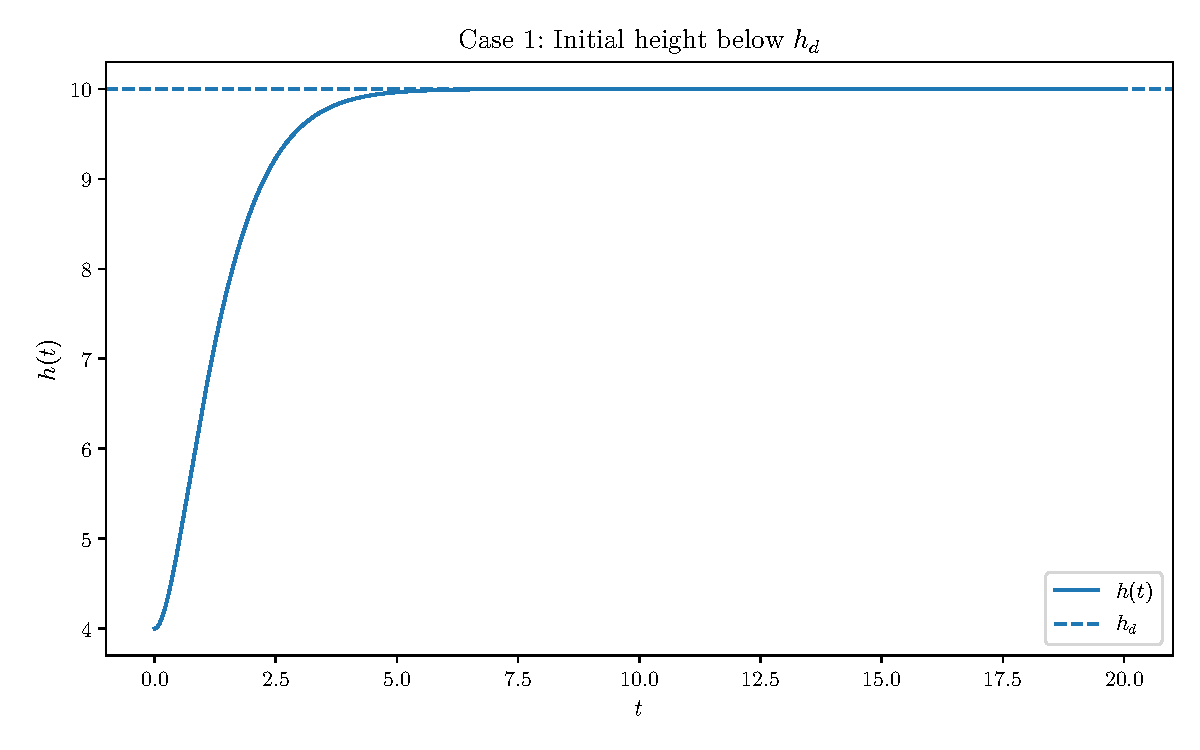
\includegraphics[scale=0.5]{figures/fig-02-02-case-01-below-hd.pdf}
\end{center}
In the first case, the body starts below the desired height:

\[
 h(0) = 4, v(0) = 0.
\]
The feedback law

\[
 u = g - k_1(h - h_d) - k_2v
\]
increases the control input because the tracking error is negative. As 
a result, the height increases and approaches $h_d$.

\begin{center}
  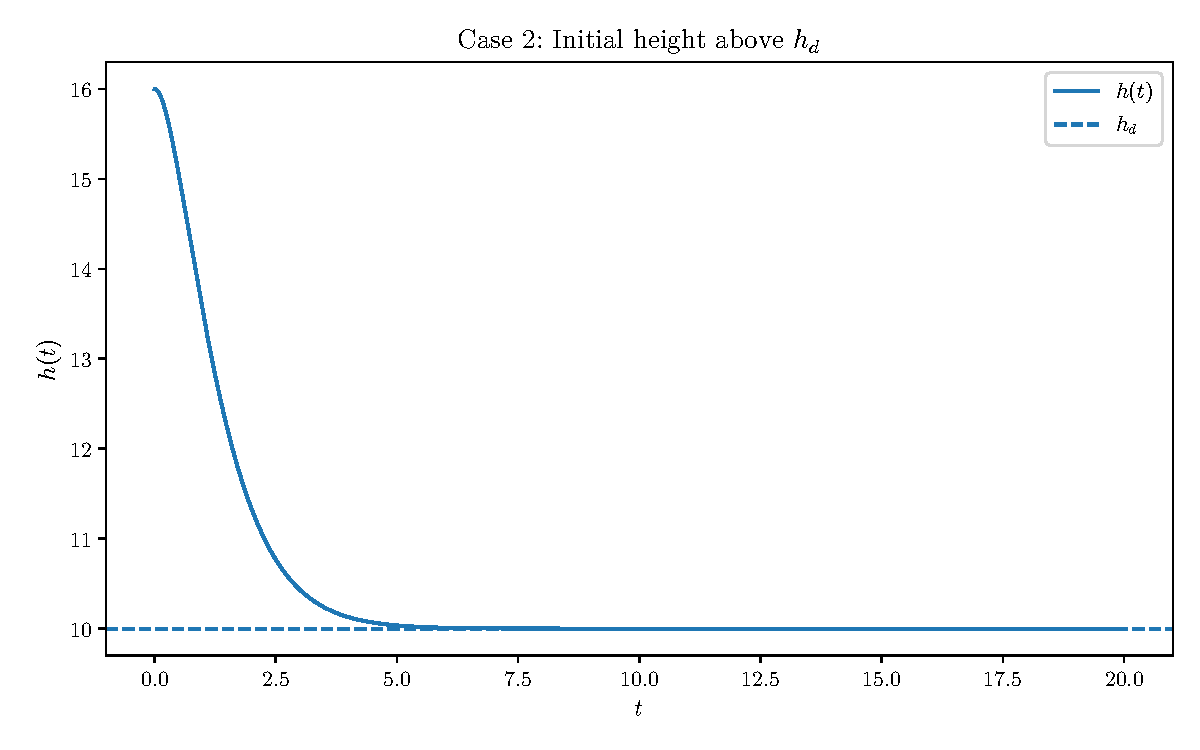
\includegraphics[scale=0.5]{figures/fig-02-02-case-02-above-hd.pdf}
\end{center}
In the second case, the body starts above the desired height:
$h(0) = 16, v(0) = 0.$ Since the tracking error is positive, the proportional feedback term decreases the control input. The height then decreases and approaches $h_d$.
\begin{center}
  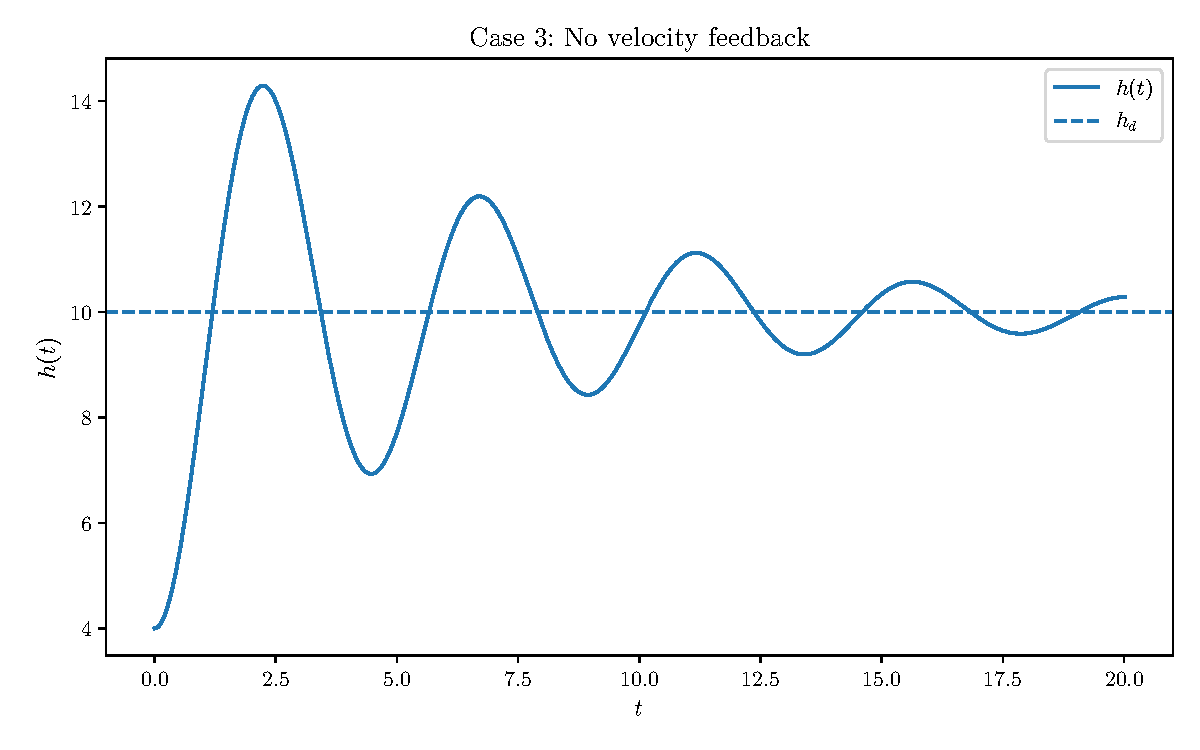
\includegraphics[scale=0.5]{figures/fig-02-02-case-03-no-velocity-feedback.pdf}
\end{center}
In the third case, we remove the velocity feedback term and use
\[
 u = g - k_1(h - h_d).
\]
This means that the controller reacts only to position error and does not directly damp the velocity. The simulation shows a stronger oscillation around $h_d$, illustrating the role of the derivative term $-k_2v$ as an additional damping mechanism.
\subsection{Stability Analysis of the CLE Equation}
\begin{theorem}
  
Let $\gamma = k_2 + c$. Rewriting~\eqref{eq:main}, we have
\begin{equation}\label{mainrewrite1}
 e''(t) + \gamma e'(t) + k_1 e(t) = 0.
\end{equation}
Suppose that $k_1 > 0$ and $\gamma > 0$. If $e(t)$ is a solution of~\eqref{mainrewrite1}, then $\limit_{t \to + \infty} e(t) = 0$.
\end{theorem}
\begin{proof} Consider the characteristic equation associated with~\eqref{mainrewrite1}:
\begin{equation}\label{characteristic}
 \lambda^2 + \gamma\lambda + k_1 = 0,
\end{equation}
The discriminant of~\eqref{characteristic} is
$\Delta = \gamma^2 - 4k_1.$
The sign of $\Delta$ determines three qualitatively different regimes.

\textbf{Case 1: $\Delta > 0$.} The characteristic equation has two distinct real roots

\[
 \lambda_1,\lambda_2 = \frac{-\gamma \pm \sqrt{\Delta}}{2}.
\]
By Vieta's formulas, we have 
\[
 \begin{cases}
 \lambda_1 + \lambda_2 = -\gamma < 0,\\
 \lambda_1\lambda_2 = k_1 > 0.
 \end{cases}
\]
Hence both roots are negative. The general solution is
\[
 e(t) = Ae^{\lambda_1 t} + Be^{\lambda_2 t},
\]
where $A, B \in \mathbb R$ are determined by the initial data. Since
$\lambda_1 < 0,\lambda_2 < 0,$ we obtain
$\limit_{t \to + \infty} e(t) = 0.$
This is the overdamped case that the error converges to zero without oscillation.

\textbf{Case 2: $\Delta = 0$.} The characteristic equation has a repeated real root
$\lambda = -\frac{\gamma}{2}.$ The general solution is
\[
 e(t) = (A + Bt)e^{-\gamma t/2}.
\]
Since $\gamma > 0$, the exponential factor $e^{-\gamma t/2}$ dominates the linear factor $A + Bt$. Therefore,
\[
 \lim_{t \to + \infty} e(t) = 0.
\]
This is the critically damped case, which lies at the boundary between non-oscillatory and oscillatory convergence.

\textbf{Case 3: $\Delta < 0$.} The characteristic roots are complex conjugates:
\[
 \lambda_{\pm} = -\frac{\gamma}{2} \pm i\omega,\quad \omega = \frac{\sqrt{4k_1 - \gamma^2}}{2}.
\]
The general real-valued solution is
\[
 e(t) = e^{-\gamma t/2} \left( A\cos(\omega t) + B\sin(\omega t) \right).
\]
Using the estimate
\[
 \left|A\cos(\omega t) + B\sin(\omega t)\right| \leq \sqrt{A^2 + B^2},
\]
we have
\[
 |e(t)| \leq \sqrt{A^2 + B^2}\, e^{-\gamma t/2} \to 0
\]
as $t \to + \infty$. Thus, $\limit_{t \to + \infty} e(t) = 0$.
\end{proof}

For example, with $k_1 = 4$, $e(0) = 3$, and $e'(0) = 0$, the three cases
$\gamma = 5, 4, 1.2$ give the overdamped, critically damped, and underdamped behaviors below.
The same RK4 implementation is used for the damping-regime comparison.
\begin{center}
  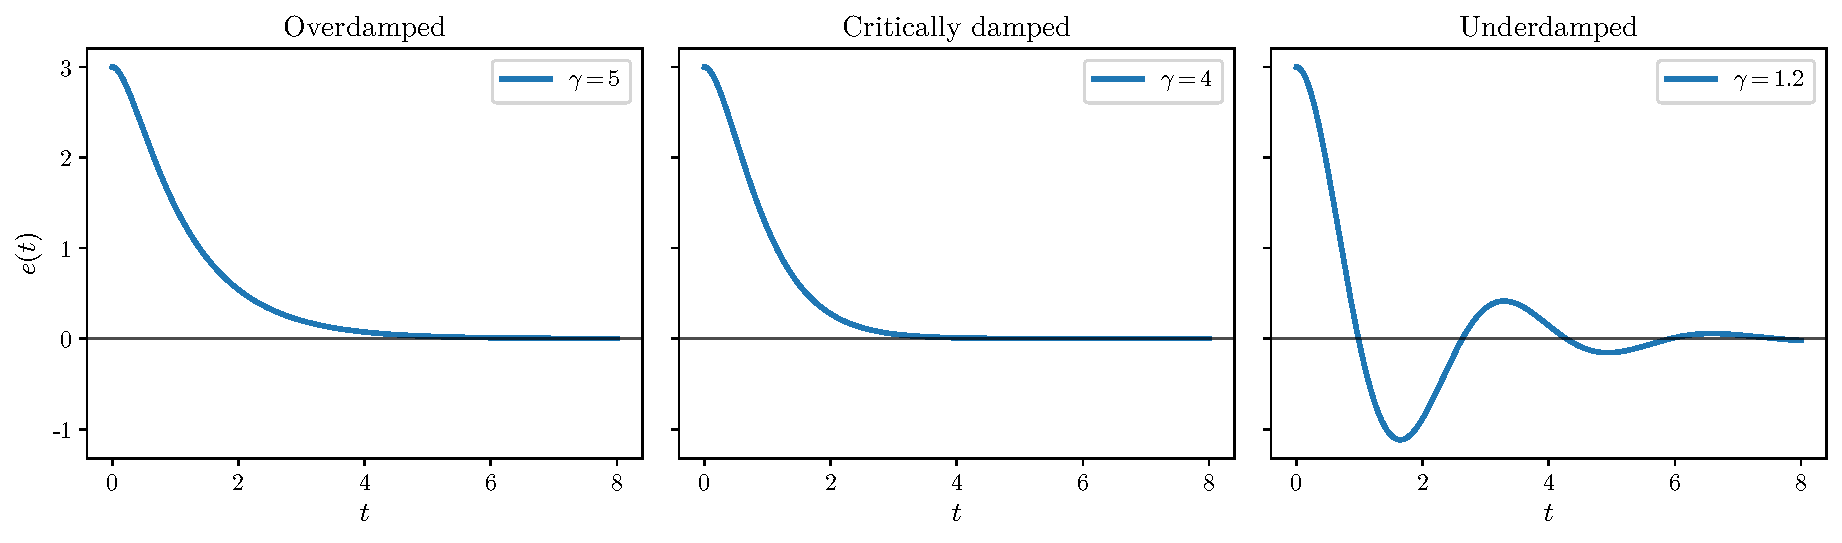
\includegraphics[scale=0.5]{figures/fig-02-05-three-regimes-side-by-side.pdf}
\end{center}

In all three cases, the assumption $k_1 > 0,\gamma = k_2 + c > 0$
guarantees that the tracking error satisfies $e(t) \to 0$.
Therefore, the height $h(t)$ approaches the desired height $h_d$. 

However, characteristic roots only describe the asymptotic behavior of the solution. They do not directly measure how much error energy remains in the system or how quickly this energy is dissipated. To study this more structurally, we introduce an energy-like quantity in the next section.
\section{Energy Method for the CLE Equation}
The notation used for the energy and variational formulation is summarized in Table~\ref{tab:energy-notation}.
\subsection{Error State Energy}
Following the Lyapunov approach to control-law design, we introduce an energy-like positive definite function and require its derivative along the controlled dynamics to be non-positive. This is the standard mechanism by which a control law is shown to stabilize the relevant error variable \cite[Sec.~5.3, pp.~59--61]{yanushevsky2019modern}. There are several requirements for such a quantity. 

First, the state of the CLE equation consists of both the tracking error $e(t)$ and its velocity $e'(t)$. Hence the quantity should measure both components. 

Second, it should be nonnegative and vanish only at the equilibrium state $e = e' = 0.$

Third, it should be compatible with the structure of equation~\eqref{mainrewrite1}. Specifically, the derivative of that quantity should contain the factor $(e'' + k_1e)$, so that the CLE equation turns it into a dissipative term.

These considerations lead to the choice
\[
 \boxed{E(t) = \frac{1}{2}(e'(t))^2 + \frac{1}{2}k_1e(t)^2.}
\]
We call this \textit{error state energy}. The first term measures the velocity part of the error, while the second term measures the position part of the error. Hence, numerically, this energy gives us how large the error state is at time $t$.
\begin{lemma}\label{decreasing}
  For all $t > 0$, one has $E'(t) = -\gamma (e'(t))^2$.
\end{lemma}
\begin{proof}
  Calculating directly and using~\eqref{mainrewrite1}, we obtain
  \begin{align*}
 E'(t) = e''(t)e'(t) + k_1 e'(t)e(t) = e'(t)(e''(t) + k_1e(t)) = e'(t) [-\gamma e'(t)]
 \end{align*}
  Hence $E'(t) = -\gamma (e'(t))^2$ for all $t > 0$.
\end{proof}

With this lemma, one can see that the error energy is non-increasing in time. Hence the CLE system does not create new error energy; instead, the damping term $\gamma e'$ dissipates it. 

To compare different feedback choices over a time interval, we introduce the \textit{accumulated error energy}
\[
 J_E(T) = \int_0^T E(t)\, dt.
\]
For the accumulated error energy over the whole time interval, we define
\[
 J_E:= \lim_{T \to + \infty} \int_0^T E(t)dt = \int_0^\infty E(t)dt.
\]
\subsection{Accumulated Control Effort}
A controller may reduce the tracking error quickly by applying a large input, but this effect is not captured by $J_E$.

To measure the amount of corrective input, one can see that the feedback law separates naturally into two parts:
\[
 u(t) = \underbrace{g}_{\text{gravity compensation}} + \underbrace{\bigl(-k_1e(t) - k_2e'(t)\bigr)}_{\text{feedback correction}}.
\]
The term $g$ is the baseline input required to compensate for gravity. Indeed, when the body is exactly at the desired height and at rest, we have

\[
 e(t) = e'(t) = 0,
\]
but the control input must still satisfy $u(t) = g$ in order to keep the body from falling. Therefore, $g$ is not part of the corrective action used to reduce the tracking error. For this reason, we measure the feedback correction beyond gravity compensation
\[
 u(t) - g = -k_1e(t) - k_2e'(t) = e''(t) + ce'(t)
\]
Then the \textit{accumulated control effort} is defined by
\[
 J_u = \int_0^T (u(t) - g)^2\, dt.
\]
This quantity measures the total size of the corrective input over the time interval $[0, T]$. If the system is already at equilibrium, then $u(t) - g = 0$, and hence $J_u = 0$, as expected for a measure of feedback correction.
\subsection{Variational Formulation of the Performance Cost}\label{VF}


The accumulated error energy $J_E$ measures how much the error state persists over time, while the accumulated control effort $J_u$ measures how much corrective input is used by the controller. To balance these two effects, we introduce the combined performance cost functional 
\[
 \boxed{ J[e] = \int_0^T \left[ \frac{1}{2}q e(t)^2 + \frac{1}{2}p(e'(t))^2 + \frac{1}{2}r(e''(t) + ce'(t))^2 \right]dt,}
\]
where $q, p, r > 0$. The first term penalizes position error, the second term penalizes velocity error, and the third term penalizes corrective control effort.

The Lagrangian is
\[
 L(e, e', e'') = \frac{1}{2}q e^2 + \frac{1}{2}p(e')^2 + \frac{1}{2}r(e'' + ce')^2.
\]
Since $L$ depends on $e''$, we use the higher-order Euler--Lagrange equation from the calculus of variations~\cite{rindler2018calculus}. We state and prove this result in Appendix~\ref{append1}. The Euler--Lagrange equation is
\[
 \frac{\partial L}{\partial e} - \frac{d}{dt}\left(\frac{\partial L}{\partial e'}\right) + \frac{d^2}{dt^2}\left(\frac{\partial L}{\partial e''}\right) = 0.
\]
We compute each term separately. First,
\[
 \frac{\partial L}{\partial e} = qe.
\]
Next, since
\[
 L = \frac{1}{2} q e^2 + \frac{1}{2} p(e')^2 + \frac{1}{2} r(e'' + ce')^2,
\]
we have
\[
 \frac{\partial L}{\partial e'} = pe' + rc(e'' + ce').
\]
Therefore,
\[
\begin{aligned}
 \frac{d}{dt}\left(\frac{\partial L}{\partial e'}\right)
 & = \frac{d}{dt} \left[ pe' + rc(e'' + ce') \right]\\
 & = pe'' + rc(e''' + ce'').
\end{aligned}
\]
Similarly,
\[
 \frac{\partial L}{\partial e''} = r(e'' + ce'),
\]
and hence
\[
\begin{aligned}
 \frac{d^2}{dt^2}\left(\frac{\partial L}{\partial e''}\right)
 & = \frac{d^2}{dt^2} \left[ r(e'' + ce')\right]\\
 & = r(e^{(4)} + ce''').
\end{aligned}
\]
Substituting these expressions into the Euler--Lagrange equation gives
\[
 qe - \left[ pe'' + rc(e''' + ce'') \right] + r(e^{(4)} + ce''') = 0.
\]
Expanding the terms, we obtain
\[
 qe - pe'' - rce''' - rc^2e'' + re^{(4)} + rce''' = 0.
\]
 Therefore,
\[
 \boxed{ re^{(4)} - (p + rc^2)e'' + qe = 0. }
\]
For a simple boundary-value formulation, one may impose
\[
 e(0) = e_0,\quad e'(0) = w_0,\quad e(T) = 0,\quad e'(T) = 0
\]

The first two conditions prescribe the initial error state, while the last two require the body to reach the desired height with zero velocity error at time $T$.
Finally, the lemma~\ref{minimizer} shows that the stationary solution of this equation is the unique global minimizer of the performance functional. 
\subsection{Compatibility with the PD feedback law}
In this section, we relate the variational weights $p, q, r$ to a compatible PD feedback law. 
The Euler--Lagrange equation associated with the variational functional is
\[
 re^{(4)} - (p + rc^2)e'' + qe = 0.
\]
Writing $D = d/dt$, this equation has the operator form
\begin{equation}\label{eq:el-operator}
 \left[rD^4 - (p + rc^2)D^2 + q\right]e = 0.
\end{equation}
On the other hand, the CLE equation generated by a PD feedback law is
\[
 e'' + \gamma e' + k_1e = 0,
\]
where
\[
 \gamma = k_2 + c.
\]
Equivalently,
\begin{equation}\label{eq:cle-operator}
 (D^2 + \gamma D + k_1)e = 0.
\end{equation}
We will use elementary algebra of constant-coefficient polynomial differential operators. 
The needed facts are collected in Appendix~\ref{appendix:operator-algebra}: polynomial operators in $D$ commute by Lemma~\ref{lem:operator-commutativity}, polynomial divisibility is equivalent to kernel inclusion by Lemma~\ref{lem:operator-kernel-inclusion}, and the quotient factor in a factorization is unique by Lemma~\ref{lem:operator-quotient-unique}.

\begin{theorem}[Factorization Theorem]\label{factor}
Assume $p, q, r > 0$, $k_1 > 0$, and $\gamma = k_2 + c > 0$.
Every solution of~\eqref{eq:cle-operator} also satisfies~\eqref{eq:el-operator} if and only if
\[
 k_1 = \sqrt{\frac{q}{r}} \quad \text{and}\quad k_2 = \sqrt{ \frac{p}{r} + c^2 + 2\sqrt{\frac{q}{r}} } - c.
\]
\end{theorem}

\begin{proof}
Let
\[
 P(\lambda) = \lambda^2 + \gamma\lambda + k_1\quad\text{and}\quad
 Q(\lambda) = r\lambda^4 - (p + rc^2)\lambda^2 + q.
\]
The compatibility condition means
$
 \ker P(D) \subseteq \ker Q(D)
$. By Lemma~\ref{lem:operator-kernel-inclusion}, this is equivalent to $P \mid Q$.
Hence there exists a polynomial $R$ such that
\[
 Q(\lambda) = R(\lambda)P(\lambda).
\]
Since $\deg Q = 4$ and $\deg P = 2$, the quotient has degree $2$. Write
\[
 R(\lambda) = r\lambda^2 + A\lambda + B.
\]Expanding the product $R(\lambda)P(\lambda)$ we obtain
\[
\begin{aligned}
 R(\lambda)P(\lambda)
 & = (r\lambda^2 + A\lambda + B)(\lambda^2 + \gamma\lambda + k_1)\\
 & = r\lambda^4 + (r\gamma + A)\lambda^3 + (rk_1 + A\gamma + B)\lambda^2\\
 &\quad + (Ak_1 + B\gamma)\lambda + Bk_1.
\end{aligned}
\]
Comparing with the polynomial
\[
 Q(\lambda) = r\lambda^4 - (p + rc^2)\lambda^2 + q = R(\lambda)P(\lambda),
\]
we obtain 
\[
 A = -r\gamma \quad \text{ and }B = rk_1.
\]
Then
\[
 r(D^2 - \gamma D + k_1)(D^2 + \gamma D + k_1) = rD^4 + r(2k_1 - \gamma^2)D^2 + rk_1^2.
\]
We compare this operator with~\eqref{eq:el-operator}:
\[
\begin{cases}
 rk_1^2 = q,\\
 r(2k_1 - \gamma^2) = -(p + rc^2).
\end{cases}
\]
Since $r > 0$, $q > 0$, and $k_1$ is taken to be a positive position-feedback gain, the first equation gives
\[
 k_1 = \sqrt{\frac{q}{r}}.
\]
From the second equation, we have
\[
 \gamma^2 = \frac{p}{r} + c^2 + 2k_1.
\]
Substituting $k_1 = \sqrt{q/r}$, we get
\[
 (k_2 + c)^2 = \gamma^2 = \frac{p}{r} + c^2 + 2\sqrt{\frac{q}{r}}.
\]
Since $\gamma > 0$, it follows that
\[
 k_2 = \sqrt{ \frac{p}{r} + c^2 + 2\sqrt{\frac{q}{r}} } - c.
\]
Conversely, if $k_1$ and $k_2$ are chosen by these formulas, then
\[
 Q(\lambda) = r(\lambda^2 - \gamma\lambda + k_1)(\lambda^2 + \gamma\lambda + k_1).
\]
Hence $P\mid Q$. By Lemma~\ref{lem:operator-kernel-inclusion}, we obtain
$\ker P(D) \subseteq \ker Q(D)$.

Therefore every solution of the CLE equation also satisfies the Euler--Lagrange equation. This completes the proof of both directions.
\end{proof}
Hence, with this choice of $k_1$ and $k_2$, every trajectory generated by the CLE equation automatically satisfies the Euler--Lagrange equation.  In simple simulations, one may fix $r = 1$ as a reference scale and tune $p$ and $q$. 
Another common approach is scale normalization. 
If the expected sizes of $e$, $e'$, and $e'' + ce'$ are $E_0$, $v_{\mathrm{start}}$, and $A_0$, respectively, then one may choose
\[
 q = \frac{1}{E_0^2},\quad p = \frac{1}{v_{\mathrm{start}}^2},\quad r = \frac{1}{A_0^2}.
\]
This makes the three terms in the performance functional comparable in size and prevents one term from dominating only because of its physical units.

\subsection{Comparing Variational and PD Responses}

In this subsection, we numerically compare several CLE trajectories. 
All trajectories are obtained by solving the CLE equation
\[
 e'' + (k_2 + c)e' + k_1e = 0.
\]
To apply the RK4 method, we rewrite this second-order equation as the first-order system
\[
 x_1 = e,\quad x_2 = e',
\]
so that
\[
\begin{cases}
 x_1' = x_2,\\
 x_2' = -(k_2 + c)x_2 - k_1x_1.
\end{cases}
\]
The RK4 method is then applied to this system with the same initial error state for all choices of $(k_1, k_2)$. For example, we choose
\[
 q = 1,\quad p = 1,\quad r = 0.2,\quad c = 0.3.
\]
Theorem~\ref{factor} yields a PD feedback law associated with these weights. Namely,
\[
 k_1 = \sqrt{\frac{q}{r}},\quad k_2 = \sqrt{ \frac{p}{r} + c^2 + 2\sqrt{\frac{q}{r}} } - c.
\]
This gives
\[
 k_1 = \sqrt{5}\approx 2.2361,\quad \text{ and }\quad k_2 = \sqrt{ 5 + 0.09 + 2\sqrt5 } - 0.3 \approx 2.7923.
\]
Thus the variational weights determine the PD feedback law
\[
 u(t) = g - k_1e(t) - k_2e'(t),
\]
with
\[
 (k_1, k_2)\approx (2.2361, 2.7923).
\]
For comparison, we also simulate three manually chosen PD feedback laws:
\[
 (k_1, k_2) = (4, 1), (4, 4), (4, 8).
\]
All trajectories start from the same initial error state
\[
 e(0) = 3,\quad e'(0) = 0,
\]
with desired height $h_d = 10$. Hence
$h(0) = h_d + e(0) = 13$.
The curve generated by
\[
 (k_1, k_2)\approx(2.2361, 2.7923)
\]
is the trajectory induced by the variational weights $p, q, r$. The other three curves are included as comparison cases. The case $k_2 = 1$ has weak damping and overshoots below the desired height. The case $k_2 = 4$ approaches $h_d$ more smoothly. The case $k_2 = 8$ is more heavily damped and remains above $h_d$ for a longer time. 
\begin{center}
    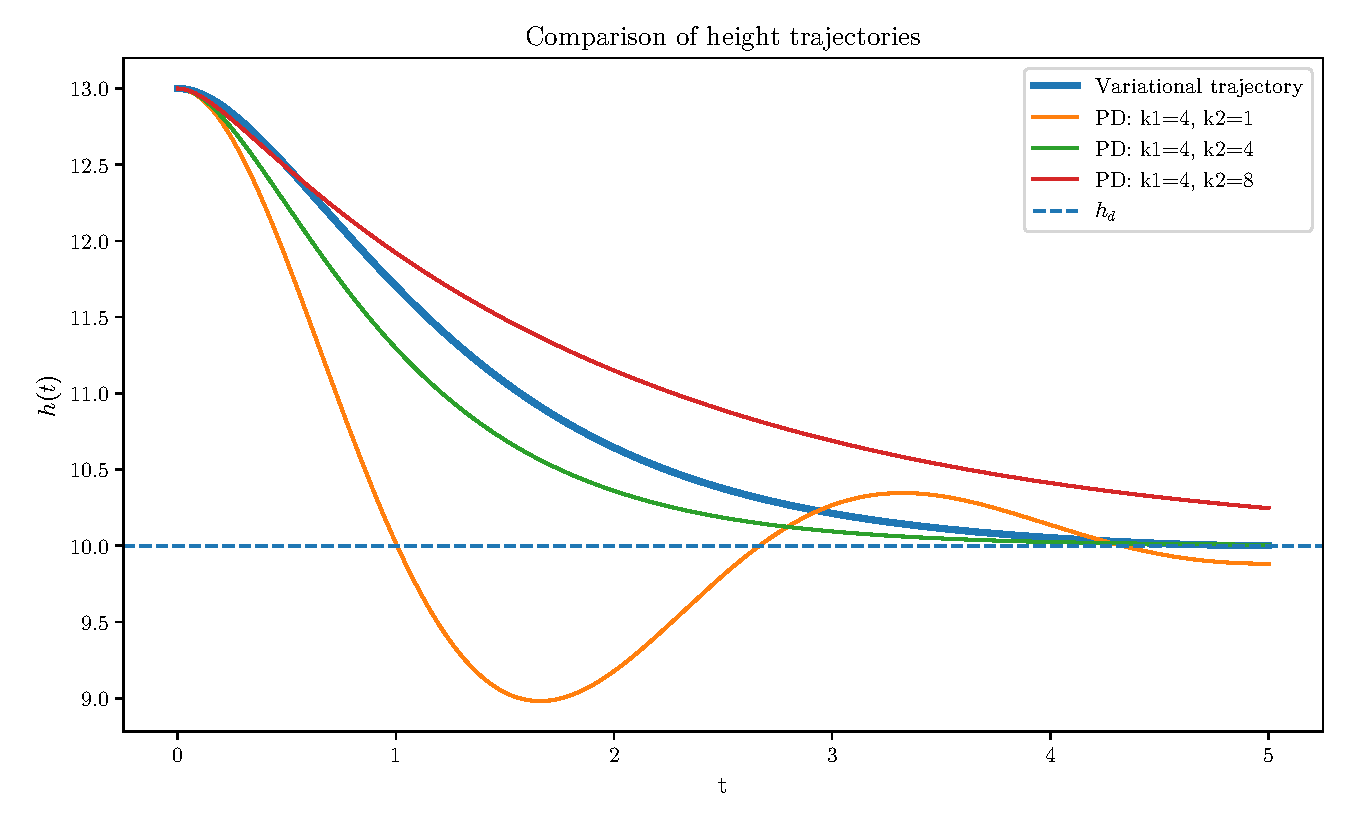
\includegraphics[scale=0.6]{figures/fig-02-07-variational-shooting.pdf}
\end{center}

\part{Mass Variation Applications}
\section{Aircraft Fuel and Mass Model}

The notation used in the simplified aircraft mass-variation model is summarized in Table~\ref{tab:fuel-notation}.

\begin{figure}[h]
\centering
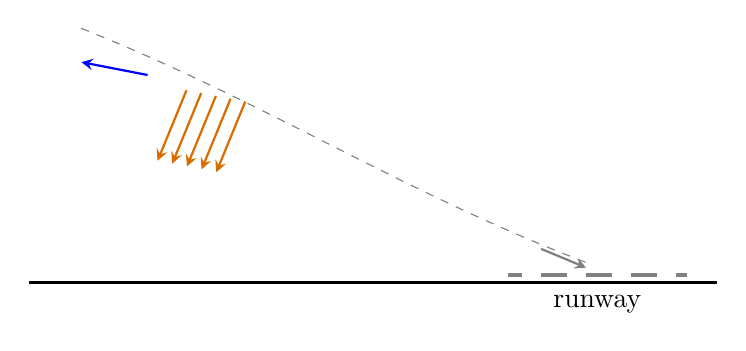
\begin{tikzpicture}[scale=0.95,>=stealth]
    % runway and descent path
    \draw[thick] (-4.6,-2.0) -- (4.6,-2.0);
    \draw[very thick,gray] (1.8,-1.9) -- (4.2,-1.9);
    \foreach \x in {2.0,2.6,3.2,3.8}
        \draw[white,line width=2pt] (\x,-1.9) -- (\x+0.25,-1.9);
    \draw[dashed,gray] (-3.9,1.4) .. controls (-1.4,0.4) and (0.4,-0.8) .. (2.9,-1.75);
    \draw[->,thick,gray] (2.25,-1.55) -- (2.85,-1.8);

    % aircraft
    \begin{scope}[shift={(-2.1,0.75)},rotate=-11]
        \node[scale=2.8] at (0,0) {\Plane};
        \draw[->,blue,thick] (-0.9,-0.15) -- (-1.8,-0.15);
        \foreach \x in {-0.35,-0.15,0.05,0.25,0.45}
            \draw[->,orange!85!black,thick] (\x,-0.25) -- (\x-0.2,-1.25);
    \end{scope}

    % fuel dump and labels
    \node[below] at (3.0,-2.05) {runway};
\end{tikzpicture}
\caption{Fuel burn and fuel dumping are modeled as mechanisms that reduce the aircraft mass during flight.}
\label{fig:aircraft-fuel-dumping}
\end{figure}
Aircraft control and simulation models commonly treat guidance and control laws as mechanisms for shaping vehicle response under simplified dynamical assumptions \cite{stevens_lewis_johnson_aircraft_control_2015}.

 Fuel burn is normally the main weight change during flight; as fuel is used, the aircraft becomes lighter and its performance is improved.

\subsection{Mass Model}
We write the total aircraft mass as
\[
 m(t) = m_{\mathrm{dry}} + m_{\mathrm{fuel}}(t).
\]
Here $m_{\mathrm{dry}}$ is the aircraft mass without usable fuel, and $m_{\mathrm{fuel}}(t)$ is the remaining fuel mass.

If fuel is consumed during flight, then $m_{\mathrm{fuel}}(t)$ decreases with time. 
Since $m_{\mathrm{dry}}$ is constant, fuel consumption gives
\[
 m'(t) = m_{\mathrm{fuel}}'(t) = -\rho(t),\quad \rho(t)\ge 0.
\]
In the constant-mass model, the 1D force balance was
\[
 m h''(t) = T(t) - mg - bh'(t).
\]
Here $m(t)$ is treated as a time-dependent parameter in the force balance. 
When the aircraft mass depends on time, this becomes
\[
 m(t)h''(t) = T(t) - m(t)g - bh'(t).
\]
Dividing by $m(t)$, we obtain
\[
 h''(t) = \frac{T(t)}{m(t)} - g - \frac{b}{m(t)}h'(t).
\]
We define
\[
 u(t) = \frac{T(t)}{m(t)},\quad c(t) = \frac{b}{m(t)}.
\]
The variable-mass equation becomes
\[
 \boxed{ h''(t) = u(t) - g - c(t)h'(t). }
\]
The constant coefficient $c$ is therefore replaced by the time-dependent coefficient
\[
 c(t) = \frac{b}{m(t)}.
\]
Thus mass loss directly changes the strength of the drag term after normalization.
\subsection{Energy Method in the Aircraft Mass Model}

In the aircraft model, the normalized drag coefficient depends on the mass profile:
\[
 c(t) = \frac{b}{m(t)}.
\]
Under the same PD feedback law
\[
 u(t) = g - k_1e(t) - k_2e'(t),
\]
the CLE equation becomes
\begin{equation}\label{cle-aircraft}
 \boxed{e''(t) + (k_2 + c(t))e'(t) + k_1e(t) = 0. }
\end{equation}
Thus the damping coefficient is no longer constant. Instead, it is given by
\[
 \gamma(t) = k_2 + c(t).
\]
We define the Lyapunov error energy by
\[
 E(t) = \frac{1}{2}(e'(t))^2 + \frac{1}{2}k_1e(t)^2.
\]
\begin{lemma}[Energy dissipation with time-dependent damping]
Suppose $k_1 > 0$, and let
\[
 \gamma(t) = k_2 + c(t).
\]
Assume that
\[
 \gamma(t)\ge \gamma(0) > 0
\]
for all $t\ge 0$. If $e$ solves~\eqref{cle-aircraft}, then one has
\[
 E(t) + \int_0^t \gamma(s)(e'(s))^2\, ds = E(0).
\]
In particular,
\[ \int_0^\infty (e'(s))^2\, ds
 \le
 \frac{E(0)}{\gamma(0)}.
\]
\end{lemma}

\begin{proof}
Differentiating $E(t)$, we get
\[
 E'(t)
 =
 e'(t)e''(t) + k_1e(t)e'(t)
 =
 e'(t)\bigl(e''(t) + k_1e(t)\bigr).
\]
Since $e$ solves
\[
 e''(t) + \gamma(t)e'(t) + k_1e(t) = 0,
\]
we have
\[
 e''(t) + k_1e(t) = -\gamma(t)e'(t).
\]
Therefore,
\begin{equation}\label{decreasingE}
 E'(t)
 =
 -\gamma(t)(e'(t))^2.
\end{equation}
    

Integrating from $0$ to $t$, we obtain
\[
 E(t) + \int_0^t \gamma(s)(e'(s))^2\, ds = E(0).
\]
Since $\gamma(s)\ge \gamma(0) > 0$, it follows that
\[
 \gamma(0) \int_0^t(e'(s))^2\, ds
 \le \int_0^t\gamma(s)(e'(s))^2\, ds
 \le
 E(0).
\]
Thus
\[ \int_0^t(e'(s))^2\, ds
 \le
 \frac{E(0)}{\gamma(0)}.
\]
Letting $t \to \infty$ gives our desired lemma.
\end{proof}
\begin{theorem}[Convergence of the aircraft CLE]
Suppose $k_1 > 0$, and suppose that the damping coefficient
$\gamma(t) = k_2 + c(t)$ satisfies
\[
 0 < \gamma_0\le \gamma(t)\le \Gamma < \infty
\]
for all $t \geq 0$. If $e$ solves~\eqref{cle-aircraft}, then $e(t) \to 0$ and $e'(t) \to 0$ as $t \to + \infty$.

\end{theorem}
\begin{proof}
For each $x > 0$, define the modified energy 
\[
 \mc{E}_x(t) = E(t) + x e(t)e'(t)
\]
where $0 < x < \sqrt{k_1}$. The next claim shows that this condition makes $\mc{E}_x(t)$ positive definite and comparable to $E(t)$.
\begin{claim}\label{4.3}
If $0 < x < \sqrt{k_1}$, then $\mathcal E_x(t)$ is equivalent to $E(t)$. More precisely,
\[
 \left(1 - \frac{x}{\sqrt{k_1}}\right)E(t)
 \le
 \mathcal E_x(t)
 \le
 \left(1 + \frac{x}{\sqrt{k_1}}\right)E(t)
\]
for all $t\ge0$.
\end{claim}
\begin{proof}[Proof of the claim]
By AM-GM inequality, one has 
\[
 |xe(t)e'(t)| = \frac{x}{\sqrt{k_1}}\left|\sqrt{k_1}e(t)\right|\left|e'(t)\right| \leq \frac{x}{\sqrt{k_1}}\left(\frac{1}{2}k_1(e(t))^2 + \frac{1}{2}(e'(t))^2\right) = \frac{x}{\sqrt{k_1}}E(t)
\]
    Then, we estimate 
\[
 \mc{E}_x(t) \leq E(t) + |xe(t)e'(t)| \leq \left(1 + \frac{x}{\sqrt{k_1}}\right)E(t)
\]
and 
\[
 \mc{E}_x(t) \geq E(t) - |xe(t)e'(t)| \geq \left(1 - \frac{x}{\sqrt{k_1}}\right)E(t)
\]
Hence, 
\[
 \left(1 - \frac{x}{\sqrt{k_1}}\right)E(t) \leq \mc{E}_x(t) \leq \left(1 + \frac{x}{\sqrt{k_1}}\right)E(t)
\]
\end{proof}
\begin{claim}\label{4.4}
    There exists $\delta > 0$ such that, for each $0 < x < \delta$, there is $a_x > 0$ satisfying
    \[
 \mc{E}'_x(t) \leq - a_x(e(t)^2 + (e'(t))^2)
 \]
    for all $t \geq 0$.
\end{claim}
\begin{proof}[Proof of the claim]
    Taking derivative yields
\begin{align*}
 \mc{E}_x'(t)
 & =
 -(\gamma(t) - x)(e'(t))^2
 -k_1x e(t)^2
 -x\gamma(t)e(t)e'(t)\\
 &\le
 -(\gamma(t) - x)(e'(t))^2
 -k_1x e(t)^2
 +x\Gamma |e(t)e'(t)|.
\end{align*}
Using AM-GM inequality
\[
 \Gamma |e(t)e'(t)|
 \le
 \frac{k_1}{2}e(t)^2
 +
 \frac{\Gamma^2}{2k_1}(e'(t))^2.
\]
Then 
\begin{align*}
 \mc{E}_x'(t)
 &\le
 -(\gamma(t) - x)(e'(t))^2
 -k_1x e(t)^2
 +
 \frac{xk_1}{2}e(t)^2
 +
 \frac{x\Gamma^2}{2k_1}(e'(t))^2\\
 & =
 -\left(\gamma(t) - x - \frac{x\Gamma^2}{2k_1}\right)(e'(t))^2
 -
 \frac{xk_1}{2}e(t)^2\\
 &\le
 -\left(\gamma_0 - x - \frac{x\Gamma^2}{2k_1}\right)(e'(t))^2
 -
 \frac{xk_1}{2}e(t)^2.
\end{align*}
    Choose
\[
 \delta = \min\left\{\sqrt{k_1},\frac{\gamma_0}{1 + \frac{\Gamma^2}{2k_1}}\right\}\quad \text{and}\quad
 a_x = \min\left\{ \gamma_0 - x - \frac{x\Gamma^2}{2k_1}, \frac{xk_1}{2}\right\}.
\]
Then for $0 < x < \delta$, we have $a_x > 0$, and we obtain 
\[
 \mc{E}'_x(t) \leq - a_x((e'(t))^2 + e(t)^2).
\]
\end{proof}
\begin{claim}
   With such $\delta > 0$ chosen above, for each fixed $0 < x < \delta$, there exists $C_x > 0$ such that
    \[
 \mc{E}'_x(t) \leq - C_x\mc{E}_x(t)
 \]
    for all $t \geq 0$.
\end{claim}
\begin{proof}[Proof of the claim]
    We have
    \[
 E(t) \leq \frac{1}{2}\max\{1, k_1\}\left(e(t)^2 + (e'(t))^2\right).
 \]
    By claim~\ref{4.3},
    \[
 E(t) \geq \frac{1}{1 + \frac{x}{\sqrt{k_1}}}\mc{E}_x(t).
 \]
    Combining together,
    \[
 e(t)^2 + (e'(t))^2 \geq \frac{2}{\max\{1, k_1\}\left(1 + \frac{x}{\sqrt{k_1}}\right)}
 \mc{E}_x(t).
 \]
    Let
    \[
 C_x
 =
 \frac{2a_x}{\max\{1, k_1\}\left(1 + \frac{x}{\sqrt{k_1}}\right)}
 > 0.
 \]
    The previous claim then gives the desired estimate.
\end{proof}
    \begin{claim}\label{4.5}
    With such $\delta > 0$ chosen above, for all $0 < x < \delta$, there exists $D_x > 0$ such that 
    \[
 \mc{E}_x(t) \leq D_xe^{-C_x t}
 \]
    \end{claim}
    for all $t \geq 0$.
    \begin{proof}[Proof of the claim]
From the previous claim, we have
\[
 \mathcal E_x'(t)\le - C_x\mathcal E_x(t)
\]
for some $C_x > 0$. This differential inequality may be viewed as a simple Grönwall-type estimate, see Appendix~\ref{gronwall}. Define
\[
 F(t) = e^{C_xt}\mathcal E_x(t).
\]
Then
\[
 F'(t)
 =
 e^{C_xt}\left(\mathcal E_x'(t) + C_x\mathcal E_x(t)\right)
 \le 0.
\]
Hence $F(t)\le F(0) = \mathcal E_x(0)$. Therefore,
\[
 e^{C_xt}\mathcal E_x(t)\le \mathcal E_x(0),
\]
which implies
\[
 \mathcal E_x(t)\le \mathcal E_x(0)e^{-C_xt}.
\]
Choosing $D_x = E_x(0)$, we obtain the desired estimate.
\end{proof}
By Claims~\ref{4.3} and~\ref{4.5}, one has
\[
 0 \leq E(t) \leq \frac{\sqrt{k_1}}{\sqrt{k_1} - x}\mc{E}_x(t) \leq \frac{\sqrt{k_1}D_x}{\sqrt{k_1} - x}e^{-C_xt}.
\]
Letting $t \to + \infty$, we obtain $E(t) \to 0$, so $e(t) \to 0$ and $e'(t) \to 0$.
\end{proof}
\section{Spacecraft Fuel and Planetary Escape}
The notation used in the simplified spacecraft model is summarized in Table~\ref{tab:spacecraft-notation}.

In the spacecraft case, the loss of mass is not only a change in the coefficient of the ODE, but also the mechanism that generates thrust.
In a simplified 1D model, we write
\[
 m(t)h''(t) = v_e(-m'(t)) - m(t)g - bh'(t),
\]
where $v_e$ is the effective exhaust velocity and $-m'(t)\ge0$ is the propellant mass flow rate during the burn. Dividing by $m(t)$, we obtain
\[
 h''(t)
 =
 v_e\frac{-m'(t)}{m(t)}
 -g
 -\frac{b}{m(t)}h'(t).
\]
Thus the spacecraft equation contains two mass-dependent effects:
\[
 v_e\frac{-m'(t)}{m(t)}
 \quad\text{and}\quad
 c(t) = \frac{b}{m(t)}.
\]
The first term is the thrust acceleration generated by propellant ejection, while the second term is the normalized drag coefficient.

\subsection{Spacecraft Propellant Mass Model}
The total mass is decomposed as
\[
 m(t) = m_{\mathrm{dry}} + m_p(t),
\]
where $m_{\mathrm{dry}}$ is the dry mass and $m_p(t)$ is the remaining propellant mass. 
During a powered burn, propellant is expelled, so
\[
 m'(t) = m_p'(t) = -\rho_p(t) < 0,
\]
where $\rho_p(t)\ge0$ is the propellant mass flow rate.

If the burn takes place on $[t_{\mathrm{start}}, t_{\mathrm{end}}]$, then the total propellant used is
\[
 m_{\mathrm{used}}
 = \int_{t_{\mathrm{start}}}^{t_{\mathrm{end}}}\rho_p(t)\, dt
 =
 m(t_{\mathrm{start}}) - m(t_{\mathrm{end}}).
\]
Thus the mass decrease during the burn is exactly the propellant mass used.
\subsection{Derivation of the Ideal Rocket Equation}

To isolate the effect of propellant mass, we consider the idealized case where gravity and drag are neglected during the burn. 
\begin{lemma}
    Suppose that, during the burn,
    \[
 h''(t)
 =
 v_e\frac{-m'(t)}{m(t)}
 \]
    with $m_{\mathrm{start}} > m_{\mathrm{end}} > 0$. Then one has 
    \[
 v_{\mathrm{end}} - v_{\mathrm{start}} = \Delta v
 =
 v_e\ln\left(\frac{m_{\mathrm{start}}}{m_{\mathrm{end}}}\right).\]
\end{lemma}
\begin{proof}
Since $v(t) = h'(t)$, we have
\[
 v'(t) = -v_e\frac{m'(t)}{m(t)}.
\]
Integrating from $t_{\mathrm{start}}$ to $t_{\mathrm{end}}$ yields
\[ \int_{t_{\mathrm{start}}}^{t_{\mathrm{end}}}v'(t)dt = \int_{t_{\mathrm{start}}}^{t_{\mathrm{end}}} - v_e\frac{m'(t)}{m(t)}dt
\]
This is equivalent to
\[ \int_{v_{\mathrm{start}}}^{v_{\mathrm{end}}}dv = -v_e \int_{m_{\mathrm{start}}}^{m_{\mathrm{end}}}\frac{1}{m}\, dm.
\]
The left-hand side is
\[ \int_{v_{\mathrm{start}}}^{v_{\mathrm{end}}}dv = v_{\mathrm{end}} - v_{\mathrm{start}}.
\]
The right-hand side is
\[
 -v_e \int_{m_{\mathrm{start}}}^{m_{\mathrm{end}}}\frac{1}{m}\, dm = -v_e \left[\ln m\right]_{m_{\mathrm{start}}}^{m_{\mathrm{end}}}.
\]
Therefore,
\[
 v_{\mathrm{end}} - v_{\mathrm{start}} = -v_e(\ln m_{\mathrm{end}} - \ln m_{\mathrm{start}}).
\]
Using the logarithm rule, this becomes
\[
 v_{\mathrm{end}} - v_{\mathrm{start}} = v_e\ln\left(\frac{m_{\mathrm{start}}}{m_{\mathrm{end}}}\right).
\]
Thus the total velocity change is
\[
 \boxed{ \Delta v = v_e\ln\left(\frac{m_{\mathrm{start}}}{m_{\mathrm{end}}}\right). }
\]
This is the ideal rocket equation~\cite{nasa_glenn_ideal_rocket_equation}. 
    
\end{proof}
\subsection{Planet Escape Criterion}

Let $R$ be the radius of the planet and let $M$ be its mass. 
We write
\[
 r(t) = R + h(t),\quad v(t) = h'(t),
\]
where $r(t)$ is the distance from the center of the planet and $h(t)$ is the altitude above the surface.

Assume that the powered burn starts at $t = t_{\mathrm{start}}$ and ends at $t = t_{\mathrm{end}}$. 
After the burn, we consider the idealized post-burn model in which the spacecraft moves only under Newtonian gravity:
\[
 h''(t) = -\frac{GM}{(R + h(t))^2},
 \quad t\ge t_{\mathrm{end}}.
\]
The corresponding mechanical energy per unit mass is
\[
 \mathcal E(t)
 =
 \frac{1}{2}v(t)^2 - \frac{GM}{R + h(t)}.
\]

\begin{lemma}[Post-burn energy conservation]
For $t\ge t_{\mathrm{end}}$, the quantity $\mathcal E(t)$ is conserved.
\end{lemma}

\begin{proof}
Differentiating $\mathcal E(t)$, we obtain
\[
\begin{aligned}
 \mathcal E'(t)
 & =
 v(t)v'(t) + \frac{GMv(t)}{(R + h(t))^2}\\
 & =
 v(t)\left(-\frac{GM}{(R + h(t))^2}\right)
 +
 \frac{GMv(t)}{(R + h(t))^2}\\
 & = 0.
\end{aligned}
\]
Hence $\mathcal E(t)$ is conserved for $t\ge t_{\mathrm{end}}$.
\end{proof}
The escape condition is expressed by the sign of the post-burn energy together with an outward post-burn velocity.
If
\[
 \mathcal E(t_{\mathrm{end}})\ge0
 \quad\text{and}\quad
 v_{\mathrm{end}}\ge0,
\]
then
\[
 \frac{1}{2}v_{\mathrm{end}}^2 - \frac{GM}{R + h_{\mathrm{end}}}\ge0.
\]
Since $v_{\mathrm{end}}\ge0$, this is equivalent to
\[
 v_{\mathrm{end}}\ge \sqrt{\frac{2GM}{R + h_{\mathrm{end}}}}.
\]
Thus the escape velocity at altitude $h_{\mathrm{end}}$ is
\[
 \boxed{
 v_{\mathrm{esc}}(h_{\mathrm{end}})
 =
 \sqrt{\frac{2GM}{R + h_{\mathrm{end}}}}.
 }
\]
\begin{figure}[h]
\centering
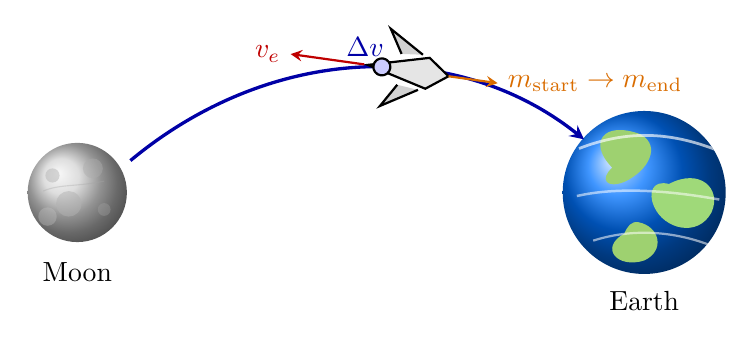
\begin{tikzpicture}[scale=0.9,>=stealth]
    % moon
    \shade[ball color=gray!35] (-4.0,0) circle (0.7);
    \begin{scope}
        \clip (-4.0,0) circle (0.7);
        \fill[gray!55,opacity=0.55] (-4.35,0.24) circle (0.10);
        \fill[gray!65,opacity=0.45] (-3.78,0.34) circle (0.14);
        \fill[gray!60,opacity=0.50] (-4.12,-0.16) circle (0.18);
        \fill[gray!70,opacity=0.35] (-3.62,-0.24) circle (0.09);
        \fill[gray!45,opacity=0.35] (-4.42,-0.34) circle (0.13);
        \draw[gray!70,opacity=0.35,line width=0.4pt] (-4.48,0.02) .. controls (-4.25,0.12) and (-4.0,0.08) .. (-3.62,0.16);
    \end{scope}

    % earth
    \shade[ball color=cyan!45!blue] (4.0,0) circle (1.15);
    \begin{scope}
        \clip (4.0,0) circle (1.15);
        \fill[green!45!brown!65] (3.55,0.35) .. controls (3.20,0.70) and (3.42,1.02) .. (3.95,0.82)
            .. controls (4.25,0.65) and (4.05,0.30) .. (3.72,0.15)
            .. controls (3.48,0.05) and (3.36,0.18) .. cycle;
        \fill[green!50!brown!60] (4.35,0.12) .. controls (4.78,0.35) and (5.10,0.06) .. (4.95,-0.28)
            .. controls (4.76,-0.64) and (4.28,-0.52) .. (4.14,-0.20)
            .. controls (4.05,0.00) and (4.12,0.18) .. cycle;
        \fill[green!45!brown!65] (3.72,-0.58) .. controls (3.36,-0.78) and (3.62,-1.08) .. (4.00,-0.96)
            .. controls (4.30,-0.82) and (4.22,-0.48) .. (3.92,-0.42)
            .. controls (3.82,-0.40) and (3.76,-0.48) .. cycle;
        \draw[white,opacity=0.65,line width=1.0pt] (3.08,0.62) .. controls (3.75,0.88) and (4.35,0.86) .. (5.02,0.60);
        \draw[white,opacity=0.55,line width=0.9pt] (3.05,-0.05) .. controls (3.62,0.08) and (4.34,0.03) .. (5.06,-0.10);
        \draw[white,opacity=0.55,line width=0.8pt] (3.28,-0.68) .. controls (3.84,-0.50) and (4.42,-0.55) .. (4.92,-0.74);
    \end{scope}
    \node[below] at (-4.0,-0.85) {Moon};
    \node[below] at (4.0,-1.25) {Earth};

    % transfer path
    \draw[->,very thick,blue!65!black]
        (-3.25,0.45) .. controls (-1.2,2.15) and (1.4,2.15) .. (3.15,0.75)
        node[midway,above] {$\Delta v$};

    % spacecraft
    \begin{scope}[shift={(0.1,1.8)},rotate=-8]
        \draw[fill=gray!20,thick] (0.0,0.0) -- (0.85,0.22) -- (1.15,0.0) -- (0.85,-0.22) -- cycle;
        \draw[fill=blue!20,thick] (0.2,0.0) circle (0.12);
        \draw[fill=gray!35,thick] (0.45,0.22) -- (0.25,0.55) -- (0.75,0.25);
        \draw[fill=gray!35,thick] (0.45,-0.22) -- (0.25,-0.55) -- (0.75,-0.25);
        \draw[->,red!75!black,thick] (-0.05,0) -- (-1.1,0)
            node[left] {$v_e$};
        \draw[->,orange!85!black,thick] (1.15,0) -- (1.85,0)
            node[right] {$m_{\mathrm{start}} \to m_{\mathrm{end}}$};
    \end{scope}
\end{tikzpicture}
\caption{A simplified spacecraft transfer from the Moon toward Earth, with propellant ejection producing the required velocity change.}
\label{fig:moon-earth-transfer}
\end{figure} 

\section{ Further Work}
Several directions remain open for further work.
First, one may replace the linear drag law by a nonlinear dissipative term. 
For example, one may consider
\[
 h'' = u - g - c(t)|h'|h'.
\]
Under the same feedback law, the corresponding error equation becomes
\[
 e'' + k_2e' + k_1e + c(t)|e'|e' = 0.
\]
The problem is to find a Lyapunov functional $\mathcal E(e, e')$ such that
\[
 \mathcal E(t)\simeq e(t)^2 + (e'(t))^2 \quad \text{ and }\quad
 \mathcal E'(t) \leq - \Phi(e'(t))
\]
for a suitable nonlinear dissipation rate $\Phi$.
Second, the spacecraft escape problem could be reformulated as a trajectory-based
optimal-control problem. One may prescribe an escape threshold
\[
 h_{\mathrm{esc}} = \alpha R,\qquad \alpha > 0.
\]
Then one may define and study the minimal escape time
\[
 \tau_{\mathrm{esc}}
 = \inf\{T_0 \geq 0: h(t) \geq h_{\mathrm{esc}}
 \text{ for all }t \geq T_0\}.
\]
For a finite-time numerical formulation, one may replace this by a sustained crossing
condition: for some observation window $\Delta T>0$,
\[
 h(t) \geq h_{\mathrm{esc}}
 \qquad
 \text{for all }t \in [T, T + \Delta T].
\]
A simplified controlled spacecraft model is
\[
\begin{cases}
 h'(t) = v(t),\\[0.3em]
 v'(t)
 =
 v_e\dfrac{\rho(t)}{m(t)}
 -
 \dfrac{GM}{(R + h(t))^2}
 -
 \dfrac{b}{m(t)}v(t),\\[0.8em]
 m'(t) = -\rho(t).
\end{cases}
\]
One possible optimal-control problem is to minimize fuel consumption subject to escape:
\[
 \min_{\rho} \int_0^T \rho(t)\, dt
\]
subject to the controlled dynamics above, the mass constraint
\[
 m(t) \geq m_{\mathrm{dry}},
\]
and the sustained crossing condition.

Third, one may formulate a data-driven version of the control problem. 
Given discrete observations
\[
 \mathcal D
 =
 \{(t_i, e_i,\dot e_i, u_i)\}_{i = 0}^{N},
\]
one may estimate the variational weights
$\theta = (p, q, r)$ or the time-dependent feedback gains $\kappa(t) = (k_1(t), k_2(t))$ from the observed dynamics.

For the variational parameters, let $e_\theta$ denote the model trajectory generated by the weights $\theta=(p,q,r)$, either through the Euler--Lagrange equation or through the compatible PD law. 
One may then consider the inverse problem
\[
 \min_{\theta \in (0, \infty)^3}
 \mathcal J_{\mathrm{data}}(\theta),
 \qquad
 \mathcal J_{\mathrm{data}}(\theta)
 =
 \sum_{i = 0}^{N}
 \left|e_\theta(t_i) - e_i\right|^2.
\]
More generally, writing $\kappa(t)=(k_1(t),k_2(t))$, the corresponding model trajectory $e_\kappa$ solves
\[
 e_\kappa''(t)
 +
 \bigl(k_2(t) + c(t)\bigr)e_\kappa'(t)
 +
 k_1(t)e_\kappa(t)
 =
 0.
\]
The associated data-fitting problem can be written as
\[
 \min_{\kappa \in \mathcal A}
 \mathcal J_{\mathrm{data}}(\kappa),
 \qquad
 \mathcal J_{\mathrm{data}}(\kappa)
 =
 \sum_{i = 0}^{N}
 \left|e_\kappa(t_i) - e_i\right|^2,
\]
where the admissible class $\mathcal A$ may impose stability constraints such as
\[
 k_1(t) \geq \kappa_0 > 0,
 \qquad
 k_2(t) + c(t) \geq \gamma_0 > 0.
\]
Since measured data may contain noise, one may add a regularization term, for example
\[
 \mathcal J_{\mathrm{reg}}(\kappa)
 =
 \mathcal J_{\mathrm{data}}(\kappa)
 +
 \lambda \int_0^T
 \left(|k_1'(t)|^2 + |k_2'(t)|^2\right)\, dt.
\]
The resulting discrete approximation could then be studied using least squares, linear programming constraints, or probabilistic filtering methods. 

Fourth, one may study forced CLE equations of the form
\[
 e'' + \gamma e' + k_1e = d(t),
\]
where $d(t)$ is an external disturbance, for instance
\[
 d(t) = \sum_{n = -N}^{N}d_ne^{in\omega t}.
\]
For a mode $e^{in\omega t}$, the operator
$
 D^2 + \gamma D + k_1
$
has multiplier
\[
 m(n) = \frac{1}{k_1 - (n\omega)^2 + i\gamma n\omega}.
\]
Hence the forced response is governed by the size of $m(n)$. 
Large values of $|m(n)|$ correspond to near-resonant frequencies, while small values correspond to strongly damped modes. 

Finally, one may extend the model from 1D motion to 3D motion. 
In this setting, the position and velocity become vector-valued:
\[
 x(t) \in \mathbb R^3,
 \qquad
 v(t) = x'(t) \in \mathbb R^3.
\]
The thrust direction is no longer fixed, so the orientation of the aircraft or spacecraft must also be modeled. 
This naturally leads to rotation groups, especially
$SO(3)$, for attitude dynamics, or more generally $SE(3) = \mathbb R^3\rtimes SO(3)$, when translation and rotation are studied together. 

\part{Technical Appendices and Notation}

\appendix
\section{Polynomial Differential Operators}\label{appendix:operator-algebra}
In this section, we collect several elementary algebraic facts about polynomial differential
operators. The background follows the course material in
\cite{le_van_luyen_la1a}.

Let $I \subset \mathbb R$ be an interval. We write
\[
 D = \frac{d}{dt}.
\]
For $j \in \mathbb N$, the notation $D^j$ means the $j$-th derivative operator:
\[
 D^j e = e^{(j)}.
\]

\begin{definition}[Polynomial differential operator]
Let
\[
 P(\lambda) = a_0 + a_1\lambda + \cdots + a_n\lambda^n
\]
be a polynomial in $\mathbb R[\lambda]$. The corresponding polynomial differential operator is defined by
\[
 P(D) = a_0 + a_1D + \cdots + a_nD^n.
\]
Thus, for a sufficiently smooth function $e$,
\[
 P(D)e
 =
 a_0e + a_1e' + \cdots + a_ne^{(n)}.
\]
\end{definition}

\begin{definition}[Polynomial divisibility]
Let $P, Q \in \mathbb R[\lambda]$ with $P \neq 0$. We say that $P$ divides $Q$, and write
\[
 P \mid Q,
\]
if there exists a polynomial $R \in \mathbb R[\lambda]$ such that
\[
 Q(\lambda) = R(\lambda)P(\lambda).
\]
The polynomial $R$ is called the quotient factor of $Q$ by $P$.
\end{definition}
\begin{lemma}[Polynomial commutativity]\label{lem:operator-commutativity}
Let $P, Q \in \mathbb R[\lambda]$, and let $P(D), Q(D)$ be the corresponding constant-coefficient polynomial differential operators. Then
\[
 P(D)Q(D) = Q(D)P(D).
\]
\end{lemma}

\begin{proof}
Write
\[
 P(\lambda) = \sum_{i = 0}^m a_i\lambda^i,
 \quad
 Q(\lambda) = \sum_{j = 0}^n b_j\lambda^j.
\]
Then
\[
 P(D)Q(D)
 =
 \left(\sum_{i = 0}^m a_iD^i\right)
 \left(\sum_{j = 0}^n b_jD^j\right)
 =
 \sum_{i = 0}^m\sum_{j = 0}^n a_ib_jD^{i + j}.
\]
Similarly,
\[
 Q(D)P(D)
 =
 \sum_{j = 0}^n\sum_{i = 0}^m b_ja_iD^{j + i}.
\]
Since $a_ib_j = b_ja_i$ and $D^{i + j} = D^{j + i}$, the two sums are equal. Hence
\[
 P(D)Q(D) = Q(D)P(D).
\]
\end{proof}

\begin{lemma}[Divisibility and kernel inclusion]\label{lem:operator-kernel-inclusion}
Let $P, Q \in \mathbb R[\lambda]$ with $P \neq 0$. 
Consider the corresponding constant-coefficient differential operators $P(D)$ and $Q(D)$, where $D = d/dt$. 
Then
$P \mid Q$ if and only if $\ker P(D) \subseteq \ker Q(D)$. Here the kernels are understood over complex-valued smooth functions. 

\end{lemma}

\begin{proof}
We prove both directions.
First, suppose $P \mid Q$. Then there exists $R \in \mathbb R[\lambda]$ such that
\[
 Q(D) = R(D)P(D).
\]
Let $e \in \ker P(D)$, then
\[
 Q(D)e
 =
 R(D)P(D)e
 =
 R(D)(0)
 =
 0.
\]
Hence $e \in \ker Q(D)$, and so $\ker P(D) \subseteq \ker Q(D)$.

Conversely, suppose $\ker P(D) \subseteq \ker Q(D)$. By polynomial division, there exist $S, T \in \mathbb R[\lambda]$ such that
\begin{equation}\label{divi1}
 Q(\lambda) = S(\lambda)P(\lambda) + T(\lambda),
 \quad
 \deg T < \deg P.
\end{equation}


\begin{claim}\label{claim1}
For every root $\alpha$ of $P$ with multiplicity $m_\alpha$, and for every integer $j$ with $0\le j\le m_\alpha - 1$, the function
\[
 e_{\alpha, j}(t) = t^j e^{\alpha t} \in \ker(D - \alpha)^{j + 1}.
\]
Consequently, we have 
\[
 e_{\alpha, j} \in \ker P(D)
\]
\end{claim}

\begin{proof}[Proof of the claim]
Write the factorization of $P$ over $\mathbb C$ as
\[
 P(\lambda) = c\prod_{\beta}(\lambda - \beta)^{m_\beta},
\]
where $c \neq 0$. Therefore,
\[
 P(D) = c\prod_{\beta}(D - \beta)^{m_\beta}.
\]
Fix a root $\alpha$ of $P$ and an integer $j$ with $0\le j\le m_\alpha - 1$. 
Since
\[
 D(t^j e^{\alpha t})
 =
 jt^{j - 1}e^{\alpha t} + \alpha t^j e^{\alpha t},
\]
we obtain
\[
 (D - \alpha)(t^j e^{\alpha t})
 =
 jt^{j - 1}e^{\alpha t}.
\]
Repeating this operation lowers the polynomial power by one each time. Hence
\[
 (D - \alpha)^{j + 1}(t^j e^{\alpha t}) = 0.
\]
Since all factors are polynomial operators in $D$ with constant coefficients, they commute. Therefore we may apply the factor $(D - \alpha)^{j + 1}$ of $P$ first, and it follows that 
\[
 e_{\alpha, j} \in \ker P(D)
\]
whenever $\alpha$ is a root of $P$ and $1 \leq j \leq m_\alpha - 1$.
\end{proof}

\begin{claim}
For every such $\alpha$ and $j$, one has $e_{\alpha, j} \in \ker T(D)$.
\end{claim} 
\begin{proof}[Proof of the claim]
By Claim~\ref{claim1}, one has $e_{\alpha, j} \in \ker P(D)$. Since we assume $\ker P(D) \subseteq \ker Q(D)$, we get
\[
 Q(D)e_{\alpha, j} = 0.
\]
From~\eqref{divi1} we obtain
\[
\begin{aligned}
 Q(D)e_{\alpha, j} = S(D)P(D)e_{\alpha, j} + T(D)e_{\alpha, j} = T(D)e_{\alpha, j} = 0
\end{aligned}
\]
\end{proof}
\begin{claim}\label{factorroot}
Let $\alpha$ be a root of $P$ with multiplicity $m_\alpha$.
If
\begin{equation}\label{assump1}
 T(D)e_{\alpha, j} = 0
 \quad
 \text{for all }0\le j\le m_\alpha - 1,
\end{equation}
then $\alpha$ is a root of $T$ with multiplicity at least $m_\alpha$. Equivalently,
\[
 \frac{d^\ell T}{d\lambda^\ell}(\alpha) = 0
 \quad
 \text{for all }0\le \ell\le m_\alpha - 1.
\]
\end{claim}
\begin{proof}[Proof of the claim]

\textbf{Step 1:} We first justify the identity
\[
 T(D)(e^{\alpha t}\phi(t))
 =
 e^{\alpha t}T(D + \alpha)\phi(t).
\]
Indeed,
\[
 D(e^{\alpha t}\phi(t))
 =
 e^{\alpha t}(\phi'(t) + \alpha\phi(t))
 =
 e^{\alpha t}(D + \alpha)\phi(t).
\]
By induction, for every $k\ge0$,
\[
 D^k(e^{\alpha t}\phi(t))
 =
 e^{\alpha t}(D + \alpha)^k\phi(t).
\]
If
\[
 T(\lambda) = \sum_{k = 0}^{N}a_k\lambda^k,
\]
then
\[
\begin{aligned}
 T(D)(e^{\alpha t}\phi(t))
 & =
 \sum_{k = 0}^{N}a_kD^k(e^{\alpha t}\phi(t))\\
 & =
 e^{\alpha t}\sum_{k = 0}^{N}a_k(D + \alpha)^k\phi(t)\\
 & =
 e^{\alpha t}T(D + \alpha)\phi(t).
\end{aligned}
\]
\textbf{Step 2: }For every integer $j\ge 0$, we will show that
\[
 T(D)(t^j e^{\alpha t})
 =
 e^{\alpha t}
 \sum_{\ell = 0}^{j}
 \binom{j}{\ell}
 \frac{d^\ell T}{d\lambda^\ell}(\alpha)
 t^{j - \ell}.
\]
Now take $\phi(t) = t^j$. By Taylor expansion of the polynomial $T$ at $\lambda = \alpha$,
\[
 T(\lambda)
 =
 \sum_{\ell = 0}^{N}
 \frac{1}{\ell!} \cdot \frac{d^\ell T}{d\lambda^\ell}(\alpha)
 (\lambda - \alpha)^\ell.
\]
Replacing $\lambda - \alpha$ by $D$, we get
\[
 T(D + \alpha)
 =
 \sum_{\ell = 0}^{N}
 \frac{1}{\ell!} \cdot \frac{d^\ell T}{d\lambda^\ell}(\alpha)
 D^\ell.
\]
Therefore, we obtain
\[
\begin{aligned}
 T(D)(t^j e^{\alpha t})
 & =
 e^{\alpha t}T(D + \alpha)t^j\\
 & =
 e^{\alpha t}
 \sum_{\ell = 0}^{j}
 \frac{1}{\ell!} \cdot \frac{d^\ell T}{d\lambda^\ell}(\alpha)
 D^\ell(t^j)\\
 & =
 e^{\alpha t}
 \sum_{\ell = 0}^{j}
 \frac{1}{\ell!} \cdot \frac{d^\ell T}{d\lambda^\ell}(\alpha)
 \frac{j!}{(j - \ell)!}t^{j - \ell}\\
 & =
 e^{\alpha t}
 \sum_{\ell = 0}^{j}
 \binom{j}{\ell}
 \frac{d^\ell T}{d\lambda^\ell}(\alpha)
 t^{j - \ell}.
\end{aligned}
\]
Here the sum stops at $\ell = j$ because $D^\ell(t^j) = 0$ for $\ell > j$. By assumption~\eqref{assump1}, we have
\[
 T(D)(t^j e^{\alpha t}) = 0.
\]
On the other hand, by the previous claim,
\[
 T(D)(t^j e^{\alpha t})
 =
 e^{\alpha t}
 \sum_{\ell = 0}^{j}
 \binom{j}{\ell}
 \frac{d^\ell T}{d\lambda^\ell}(\alpha)
 t^{j - \ell}.
\]
Therefore,
\[
 e^{\alpha t}
 \sum_{\ell = 0}^{j}
 \binom{j}{\ell}
 \frac{d^\ell T}{d\lambda^\ell}(\alpha)
 t^{j - \ell}
 =
 0
\]
for all $t$. Since $e^{\alpha t} \neq 0$ for all $t$, it follows that
\[
 \sum_{\ell = 0}^{j}
 \binom{j}{\ell}
 \frac{d^\ell T}{d\lambda^\ell}(\alpha)
 t^{j - \ell}
 \equiv 0.
\]
\textbf{Step 3:} We now prove the desired conclusion by induction on $j$.

For each $j$ with $0\le j\le m_\alpha - 1$, define
\[
 A_j:=
 \frac{d^jT}{d\lambda^j}(\alpha).
\]
The polynomial identity obtained above (and~\eqref{assump1}) becomes
\[
 \sum_{\ell = 0}^{j}\binom{j}{\ell}A_\ell t^{j - \ell}\equiv0.
\]
This gives a triangular recurrence for the coefficients $A_j$.
For $j = 0$, the identity is simply
\[
 A_0 = T(\alpha) = 0.
\]
Now suppose that $1\le j\le m_\alpha - 1$ and that
\[
 A_0 = A_1 = \cdots = A_{j - 1} = 0.
\]
For this value of $j$, the identity is
\[
 \binom{j}{0}A_0t^j
 +
 \binom{j}{1}A_1t^{j - 1}
 + \cdots
 +
 \binom{j}{j - 1}A_{j - 1}t
 +
 A_j
 \equiv0.
\]
By the induction hypothesis, all terms except the last one vanish. Hence
$A_j = 0$.
Therefore, by induction,
\[
 A_\ell = 0
 \quad
 \text{for all }0\le \ell\le m_\alpha - 1.
\]
Equivalently,
\[
 \frac{d^\ell T}{d\lambda^\ell}(\alpha) = 0
 \quad
 \text{for all }0\le \ell\le m_\alpha - 1.
\]
\end{proof}
By Claim~\eqref{factorroot}, every root $\alpha$ of $P$ is also a root of $T$ with multiplicity at least $m_\alpha$. Therefore,
$
 P \mid T
$ over $\mathbb C[\lambda]$. But from polynomial division,
$
 \deg T < \deg P
$. Hence, the only possibility is $T = 0$.

Therefore, $Q(\lambda) = S(\lambda)P(\lambda)$. The proof is complete.
\end{proof}
\begin{lemma}[Uniqueness of quotient factor]\label{lem:operator-quotient-unique}
    Suppose $P, Q \in \mathbb R[\lambda]$ with $P \neq 0$ and $P \mid Q$. Then the quotient factor of $Q$ by $P$ is unique.
\end{lemma}

\begin{proof}
    Suppose there are $R_1, R_2 \in \mathbb R[\lambda]$ such that
    \[
 Q(\lambda) = R_1(\lambda)P(\lambda) = R_2(\lambda)P(\lambda).
 \]
    Then
    \[
 (R_1(\lambda) - R_2(\lambda))P(\lambda) = 0.
 \]
    We prove that $R_1(\lambda) - R_2(\lambda) = 0$ by contradiction. Suppose instead that
    \[
 R_1(\lambda) - R_2(\lambda) \neq 0.
 \]
    Since $P(\lambda) \neq 0$, both $P(\lambda)$ and $R_1(\lambda) - R_2(\lambda)$ are nonzero polynomials.
    Let $m = \deg P$ and  $n = \deg(R_1 - R_2)$. Write the leading terms as
    \[
 P(\lambda) = a_m\lambda^m + \text{lower - order terms},
 \]
    and
    \[
 R_1(\lambda) - R_2(\lambda) = b_n\lambda^n + \text{lower - order terms},
 \]
    where $a_m \neq 0$ and $b_n \neq 0$.

    Then the leading term of $(R_1 - R_2)P$ is $a_mb_n\lambda^{m + n}$.
    Since $a_m \neq 0$ and $b_n \neq 0$, and since $\mathbb R$ has no zero divisors, we have
    \[
 a_mb_n \neq 0.
 \]
    Hence
    \[
 (R_1(\lambda) - R_2(\lambda))P(\lambda)
 \]
    is not the zero polynomial, contradicting
    \[
 (R_1(\lambda) - R_2(\lambda))P(\lambda) = 0.
 \]
    Therefore,
    \[
 R_1(\lambda) - R_2(\lambda) = 0.
 \]
    Hence
    \[
 R_1(\lambda) = R_2(\lambda).
 \]
    Therefore the quotient factor of $Q$ by $P$ is unique.
\end{proof}

\section{Laplace Transform and Characteristic Roots}
\label{appendix:laplace-characteristic}

In this appendix, we recall the basic Laplace transform identities needed to justify the characteristic-root formulas used in the stability analysis.

\begin{definition}[Laplace transform]
Let $f:[0, \infty) \to \mathbb R$ be a function such that the integral below exists for $s$ sufficiently large. The Laplace transform of $f$ is defined by
\[
 \mathcal L[f](s)
 = \int_0^\infty e^{-st}f(t)\, dt.
\]
When no confusion is possible, we write
\[
 F(s) = \mathcal L[f](s).
\]
\end{definition}

\begin{lemma}[Linearity]
If $\mathcal L[f]$ and $\mathcal L[g]$ exist, then for any constants $a, b \in \mathbb R$,
\[
 \mathcal L[af + bg](s)
 =
 a\mathcal L[f](s) + b\mathcal L[g](s).
\]
\end{lemma}

\begin{proof}
By the linearity of the integral,
\[
\begin{aligned}
 \mathcal L[af + bg](s)
 & = \int_0^\infty e^{-st}(af(t) + bg(t))\, dt\\
 & =
 a \int_0^\infty e^{-st}f(t)\, dt
 +
 b \int_0^\infty e^{-st}g(t)\, dt\\
 & =
 a\mathcal L[f](s) + b\mathcal L[g](s).
\end{aligned}
\]
\end{proof}

\begin{lemma}[Laplace transform of derivatives]
Suppose $f$ is sufficiently smooth and of exponential order so that the following transforms exist. If $F(s) = \mathcal L[f](s)$, then
\[
 \mathcal L[f'](s) = sF(s) - f(0),
\]
and
\[
 \mathcal L[f''](s) = s^2F(s) - sf(0) - f'(0).
\]
\end{lemma}

\begin{proof}
By integration by parts,
\[
\begin{aligned}
 \mathcal L[f'](s)
 & = \int_0^\infty e^{-st}f'(t)\, dt\\
 & =
 \left[e^{-st}f(t)\right]_0^\infty
 +
 s \int_0^\infty e^{-st}f(t)\, dt.
\end{aligned}
\]
Under the assumption that $e^{-st}f(t) \to 0$ as $t \to \infty$, we obtain
\[
 \left[e^{-st}f(t)\right]_0^\infty
 =
 0 - f(0)
 =
 -f(0).
\]
Hence
\[
 \mathcal L[f'](s) = sF(s) - f(0).
\]
Applying the same formula to $f'$, we get
\[
 \mathcal L[f''](s)
 =
 s\mathcal L[f'](s) - f'(0).
\]
Using the first identity, we obtain
\[
 \mathcal L[f''](s) = s^2F(s) - sf(0) - f'(0).
\]
\end{proof}

\begin{lemma}[Basic Laplace transforms]
For constants $a \in \mathbb R$ and $\omega > 0$, one has
\[
 \mathcal L[e^{at}](s) = \frac{1}{s - a},
\]
\[
 \mathcal L[te^{at}](s) = \frac{1}{(s - a)^2},
\]
\[
 \mathcal L[e^{at}\cos(\omega t)](s)
 =
 \frac{s - a}{(s - a)^2 + \omega^2},
\]
and
\[
 \mathcal L[e^{at}\sin(\omega t)](s)
 =
 \frac{\omega}{(s - a)^2 + \omega^2}.
\]
\end{lemma}
\begin{proof}
For $s > a$,
\[
 \mathcal L[e^{at}](s)
 = \int_0^\infty e^{-st}e^{at}\, dt
 = \int_0^\infty e^{-(s - a)t}\, dt
 =
 \frac{1}{s - a}.
\]
Next,
\[
 \mathcal L[te^{at}](s)
 = \int_0^\infty t e^{-(s - a)t}\, dt.
\]
Using integration by parts with $u = t$ and $dv = e^{-(s - a)t}dt$, we get
\[ \int_0^\infty t e^{-(s - a)t}\, dt
 =
 \frac{1}{(s - a)^2}.
\]
Thus
\[
 \mathcal L[te^{at}](s) = \frac{1}{(s - a)^2}.
\]
For the trigonometric formulas, use
\[
 e^{at}\cos(\omega t) = \operatorname{Re}\left(e^{(a + i\omega)t}\right),
\]
and
\[
 e^{at}\sin(\omega t) = \operatorname{Im}\left(e^{(a + i\omega)t}\right).
\]
Since
\[
 \mathcal L[e^{(a + i\omega)t}](s)
 =
 \frac{1}{s - a - i\omega}
 =
 \frac{s - a + i\omega}{(s - a)^2 + \omega^2},
\]
taking real and imaginary parts gives
\[
 \mathcal L[e^{at}\cos(\omega t)](s)
 =
 \frac{s - a}{(s - a)^2 + \omega^2},
\]
and
\[
 \mathcal L[e^{at}\sin(\omega t)](s)
 =
 \frac{\omega}{(s - a)^2 + \omega^2}.
\]
\end{proof}
The characteristic-root analysis of constant-coefficient linear ODEs follows the standard qualitative theory of differential equations \cite{kelley_peterson_ode_2010}.
\begin{theorem}[Characteristic solutions]
Consider the equation
\[
 e''(t) + \gamma e'(t) + k_1e(t) = 0,
\]
with initial data
\[
 e(0) = e_0,\quad e'(0) = w_0.
\]
Let
\[
 \Delta = \gamma^2 - 4k_1.
\]
Then the solution has the following forms:
\[
\begin{cases}
 e(t) = Ae^{\lambda_1t} + Be^{\lambda_2t}, & \Delta > 0,\\[4pt]
 e(t) = (A + Bt)e^{\lambda t}, & \Delta = 0,\\[4pt]
 e(t) = e^{\alpha t}\left(A\cos(\omega t) + B\sin(\omega t)\right), & \Delta < 0,
\end{cases}
\]
where
\[
 \lambda_1 = \frac{-\gamma + \sqrt{\Delta}}2,
 \quad
 \lambda_2 = \frac{-\gamma - \sqrt{\Delta}}2,
 \quad
 \lambda = -\frac{\gamma}{2},
 \quad
 \alpha = -\frac{\gamma}{2},
 \quad
 \omega = \frac{\sqrt{4k_1 - \gamma^2}}2.
\]
\end{theorem}
\begin{proof}
Let $E(s) = \mathcal L[e](s)$. Taking the Laplace transform of
\[
 e'' + \gamma e' + k_1e = 0,
\]
and using the derivative identities above, we obtain
\[
 s^2E(s) - se_0 - w_0 + \gamma(sE(s) - e_0) + k_1E(s) = 0.
\]
Hence
\[
 (s^2 + \gamma s + k_1)E(s) = (s + \gamma)e_0 + w_0.
\]
Therefore
\[
 E(s) = \frac{(s + \gamma)e_0 + w_0}{s^2 + \gamma s + k_1}.
\]
Thus the form of the solution is determined by the factorization of $s^2 + \gamma s + k_1$.
\begin{claim}
If $\Delta > 0$, then the solution has the form
\[
 e(t) = Ae^{\lambda_1t} + Be^{\lambda_2t}.
\]
\end{claim}
\begin{proof}[Proof of the claim]
If $\Delta > 0$, then
\[
 s^2 + \gamma s + k_1 = (s - \lambda_1)(s - \lambda_2),
\]
where
\[
 \lambda_1 = \frac{-\gamma + \sqrt{\Delta}}2,
 \quad
 \lambda_2 = \frac{-\gamma - \sqrt{\Delta}}2.
\]
Thus
\[
 E(s)
 =
 \frac{(s + \gamma)e_0 + w_0}{(s - \lambda_1)(s - \lambda_2)}.
\]
By partial fractions, there exist constants $A, B \in \mathbb R$ such that
\[
 E(s) = \frac{A}{s - \lambda_1} + \frac{B}{s - \lambda_2}.
\]
Taking inverse Laplace transforms gives
\[
 e(t) = Ae^{\lambda_1t} + Be^{\lambda_2t}.
\]
\end{proof}
\begin{claim}
If $\Delta = 0$, then the solution has the form
\[
 e(t) = (A + Bt)e^{\lambda t}.
\]
\end{claim}
\begin{proof}[Proof of the claim]
If $\Delta = 0$, then the characteristic root is 
\[
 \lambda = -\frac{\gamma}{2}.
\]
Hence
\[
 s^2 + \gamma s + k_1 = (s - \lambda)^2.
\]
Therefore
\[
 E(s) = \frac{(s + \gamma)e_0 + w_0}{(s - \lambda)^2}.
\]
Since
\[
 (s + \gamma)e_0 + w_0
 =
 e_0(s - \lambda)
 +
 \left(w_0 + \frac{\gamma}{2}e_0\right),
\]
we get
\[
 E(s)
 =
 \frac{e_0}{s - \lambda}
 +
 \frac{w_0 + \frac{\gamma}{2}e_0}{(s - \lambda)^2}.
\]
Taking inverse Laplace transforms gives
\[
 e(t)
 =
 e_0e^{\lambda t}
 +
 \left(w_0 + \frac{\gamma}{2}e_0\right)te^{\lambda t}.
\]
Thus the solution has the form
\[
 e(t) = (A + Bt)e^{\lambda t}.
\]
\end{proof}
\begin{claim}
If $\Delta < 0$, then the solution has the form
\[
 e(t) = e^{\alpha t}\left(A\cos(\omega t) + B\sin(\omega t)\right).
\]
\end{claim}
\begin{proof}[Proof of the claim]
Finally, suppose $\Delta < 0$. Define
\[
 \alpha = -\frac{\gamma}{2},
 \quad
 \omega = \frac{\sqrt{4k_1 - \gamma^2}}2.
\]
Then
\[
 s^2 + \gamma s + k_1 = (s - \alpha)^2 + \omega^2.
\]
Therefore
\[
 E(s) = \frac{(s + \gamma)e_0 + w_0}{(s - \alpha)^2 + \omega^2}.
\]
Since
\[
 (s + \gamma)e_0 + w_0
 =
 e_0(s - \alpha)
 +
 \left(w_0 + \frac{\gamma}{2}e_0\right),
\]
we obtain
\[
 E(s)
 =
 e_0\frac{s - \alpha}{(s - \alpha)^2 + \omega^2}
 +
 \left(w_0 + \frac{\gamma}{2}e_0\right)
 \frac{1}{(s - \alpha)^2 + \omega^2}.
\]
Using the basic inverse Laplace transforms,
\[
 \mathcal L^{-1}\left[
 \frac{s - \alpha}{(s - \alpha)^2 + \omega^2}
 \right]
 =
 e^{\alpha t}\cos(\omega t),
\]
and
\[
 \mathcal L^{-1}\left[
 \frac{\omega}{(s - \alpha)^2 + \omega^2}
 \right]
 =
 e^{\alpha t}\sin(\omega t),
\]
we get
\[
 e(t)
 =
 e^{\alpha t}
 \left[
 e_0\cos(\omega t)
 +
 \frac{w_0 + \frac{\gamma}{2}e_0}{\omega}\sin(\omega t)
 \right].
\]
Thus the solution has the form
\[
 e(t) = e^{\alpha t}\left(A\cos(\omega t) + B\sin(\omega t)\right).
\]
\end{proof}
The proof is complete.
\end{proof}

\section{Calculus of Variations}
\subsection{First Fundamental Lemma of Variation}
The bump-function construction follows the standard smooth cutoff construction in~\cite{lee_smooth_manifolds}.
\begin{lemma}[Smooth bump function]
Let $I = (t_0 - \delta, t_0 + \delta)$ be an interval such that
\[
 [t_0 - \delta, t_0 + \delta] \subset (a, b).
\]
Define
\[
\eta(t) =
\begin{cases}
\exp\left(-\dfrac{1}{\delta^2 - (t - t_0)^2}\right),
& |t - t_0| < \delta,\\[1em]
0,
& |t - t_0| \geq \delta.
\end{cases}
\]
Then
\[
 \eta \in C_c^\infty((a, b)),\quad \eta(t) \geq 0 \text{ for all }t,
\]
and $\eta(t) > 0$ if and only if $t \in I$.
\end{lemma}

\begin{proof}
We divide the proof into several claims.

\begin{claim}\label{C.4}
One has $\eta(t) \geq 0$ for all $t$, and $\eta(t) > 0$ if and only if $t \in I$.
\end{claim}

\begin{proof}[Proof of the claim]
If $|t - t_0| < \delta$, then
\[
 \delta^2 - (t - t_0)^2 > 0.
\]
Hence
\[
 \eta(t)
 =
 \exp\left(-\frac{1}{\delta^2 - (t - t_0)^2}\right) > 0.
\]
If $|t - t_0| \geq \delta$, then $\eta(t) = 0$. Therefore $\eta(t) \geq 0$ for all $t$, and $\eta(t) > 0$ precisely when $t \in I$.
\end{proof}

\begin{claim}\label{C.5}
The support of $\eta$ is
\[
 \operatorname{supp}\eta = [t_0 - \delta, t_0 + \delta].
\]
In particular, $\operatorname{supp}\eta$ is compactly contained in $(a, b)$.
\end{claim}

\begin{proof}[Proof of the claim]
From the previous claim, $\eta(t) > 0$ exactly on
\[
 I = (t_0 - \delta, t_0 + \delta),
\]
and $\eta(t) = 0$ outside $I$. Hence
\[
 \{t:\eta(t) \neq 0\} = I.
\]
Therefore
\[
 \operatorname{supp}\eta
 =
 \overline{\{t:\eta(t) \neq 0\}}
 =
 \overline I
 =
 [t_0 - \delta, t_0 + \delta].
\]
By assumption,
\[
 [t_0 - \delta, t_0 + \delta] \subset (a, b),
\]
so the support is compactly contained in $(a, b)$.
\end{proof}
\begin{claim}\label{C.6}
The function $\eta$ is smooth at the boundary points $t = t_0 \pm \delta$.
\end{claim}
\begin{proof}[Proof of the claim]
Inside $I$, put
$
 s = \delta^2 - (t - t_0)^2.
$
Then $s > 0$ on $I$, and $s \to 0^+$ as $t \to t_0 \pm \delta,\ t \in I$.
We first describe the form of the higher derivatives. Since $s$ is a polynomial in $t$, repeated differentiation of $e^{-1/s}$ gives, for each $k \geq 0$,
\[
 \eta^{(k)}(t)
 =
 \sum_i C_i(t)s^{-N_i}e^{-1/s}
\]
on $I$, where each $N_i$ is a nonnegative integer and each $C_i(t)$ is bounded near $t = t_0 \pm \delta$. 
It remains to show that every term of this form tends to $0$. For every $N \in \mathbb N$, one has
\[
 \lim_{s \to 0^+}s^{-N}e^{-1/s} = 0.
\]
Indeed, setting $u = 1/s$, we have $u \to + \infty$ and
\[
 s^{-N}e^{-1/s} = u^Ne^{-u} \to 0.
\]
Therefore every term $C_i(t)s^{-N_i}e^{-1/s}$ tends to $0$ as $t \to t_0 \pm \delta$ from inside $I$. Hence
\[
 \lim_{t \to t_0 \pm \delta,\ t \in I}\eta^{(k)}(t) = 0
\]
for every $k \geq 0$.

Outside $I$, we have $\eta\equiv0$, so every derivative is also zero there. Thus all one-sided derivatives agree at $t = t_0 \pm \delta$, and all of them are equal to $0$. Therefore $\eta$ is smooth at the boundary points.
\end{proof}

\begin{claim}\label{C.7}
One has $\eta \in C^\infty((a, b))$.
\end{claim}

\begin{proof}[Proof of the claim]
On the open interval $I$, the function is a composition of smooth functions:
\[
 \eta(t) = \exp\left(-\frac{1}{\delta^2 - (t - t_0)^2}\right),
\]
so $\eta$ is smooth on $I$.

On $(a, b)\setminus [t_0 - \delta, t_0 + \delta]$, we have $\eta\equiv0$, so $\eta$ is smooth there. By the previous claim, $\eta$ is also smooth at the boundary points $t = t_0 \pm \delta$. Hence
$
 \eta \in C^\infty((a, b)).
$
\end{proof}
    By Claims~\ref{C.4},~\ref{C.5},~\ref{C.6} and~\ref{C.7}, the function $\eta$ is nonnegative, positive precisely on $I$, smooth on $(a, b)$, and compactly supported in $(a, b)$. Hence
\[
 \eta \in C_c^\infty((a, b)).
\]
This proves the lemma.
\end{proof}
    \begin{lemma}[First Fundamental Lemma]\label{FFL}
        Suppose $F \in C([a, b])$ and one has 
        \[ \int_a^b F(t)\eta(t)dt = 0
 \]
        for all test functions $\eta \in C_c^\infty((a, b))$, then $F \equiv 0$ on $(a, b)$.
    \end{lemma}
    \begin{proof}[Proof of the lemma]
        Suppose there is $t_0 \in (a, b)$ such that $F(t_0) \neq 0$, one can assume that $F(t_0) > 0$. Since $F$ is continuous, there exists $\delta > 0$ such that $F(t) > 0$ for all $t \in (t_0 - \delta, t_0 + \delta)$. Choose $\eta \in C_c^\infty((a, b))$ as constructed in the previous lemma with $\eta \geq 0$ for all $t \in (a, b)$ and $\eta > 0$ if and only if $t \in (t_0 - \delta, t_0 + \delta)$. This gives
            \[
 0 = \int_a^b F(t)\eta(t)\, dt = \int_{t_0 - \delta}^{t_0 + \delta}F(t)\eta(t)\, dt > 0,
 \]
            which is impossible.
        If $F(t_0) < 0$, the argument is similar.
    \end{proof}
\subsection{Euler--Lagrange Equation}\label{append1}

\begin{theorem}[Higher-order Euler--Lagrange equation]
Let $a < b$, and let
\[
 L:[a, b] \times \mathbb{R}^3 \to \mathbb{R}
\]
be $C^2$. Consider the functional
\[
 J[y] = \int_a^b L(t, y(t), y'(t), y''(t))\, dt
\]
on the admissible class
\[
 \mathcal A = \left\{ y \in C^2([a, b]): y(a) = A,\ y'(a) = B,\ y(b) = C,\ y'(b) = D \right\}.
\]
Suppose that $y \in \mathcal A$ is a stationary point of $J$, meaning that for every
$\eta \in C_c^\infty((a, b))$ satisfying
\begin{equation}\label{testfunction}
\eta(a) = \eta'(a) = \eta(b) = \eta'(b) = 0,
\end{equation}
one has
\[
 \left.\frac{d}{d\varepsilon}J[y + \varepsilon\eta]\right|_{\varepsilon = 0} = 0.
\]
Then $y$ satisfies the higher-order Euler--Lagrange equation
\[
\boxed{
\begin{aligned}
\frac{\partial L}{\partial y}
-
\frac{d}{dt}\left(\frac{\partial L}{\partial y'}\right)
+
\frac{d^2}{dt^2}\left(\frac{\partial L}{\partial y''}\right)
 = 0
\end{aligned}
}
\]
on $(a, b)$.
\end{theorem} 
\begin{proof}
    \begin{claim}Let $y \in \mc{A}$ be a stationary point of $J$, and let $\eta \in C_c^\infty((a, b))$ be any test function satisfying~\eqref{testfunction}. One has 
            \[ \int_a^b \eta\left[\frac{dL}{dy} - \frac{d}{dt}\left(\frac{dL}{dy'}\right) + \frac{d^2}{dt^2}\left(\frac{dL}{dy''}\right)\right] dt = 0
 \]
    \end{claim}
    \begin{proof}[Proof of the claim] Define $\Phi(\ep) = J[y + \ep\eta]$, then we have 
    \begin{equation}\label{euler1}
 \Phi'(0) = \frac{d}{d\ep}J[y + \ep\eta]\bigg|_{\ep = 0} = \int_a^b \frac{d}{d\ep} L(t, y + \ep\eta, y' + \ep\eta', y'' + \ep\eta'')\bigg|_{\ep = 0}dt = 0
 \end{equation}
    By the chain rule,
    \[
 \frac{d}{d\varepsilon} L(t, y + \varepsilon\eta, y' + \varepsilon\eta', y'' + \varepsilon\eta'') = L_y\eta + L_{y'}\eta' + L_{y''}\eta'',
 \]
    where the partial derivatives are evaluated at
    \[
 (t, y + \varepsilon\eta, y' + \varepsilon\eta', y'' + \varepsilon\eta'').
 \]
    Evaluating at $\varepsilon = 0$, we obtain
    \[
 \left. \frac{d}{d\varepsilon} L(t, y + \varepsilon\eta, y' + \varepsilon\eta', y'' + \varepsilon\eta'') \right|_{\varepsilon = 0} = L_y\eta + L_{y'}\eta' + L_{y''}\eta'',
 \]
    where now the derivatives are evaluated along
    \[
 (t, y(t), y'(t), y''(t)).
 \]
     Substituting this into the right-hand side of~\eqref{euler1}, we obtain 
    \begin{equation}\label{euler2} \int_a^b \left( \eta\frac{dL}{dy} + \eta'\frac{dL}{dy'} + \eta''\frac{dL}{dy''}\right)dt = 0
 \end{equation}
    Applying integration by parts to the last two terms gives
    \[ \int_a^b \eta'\frac{dL}{dy'} dt = \left( \eta \frac{dL}{dy'}\right)\bigg|_a^b - \int_a^b \eta \frac{d}{dt}\left(\frac{dL}{dy'}\right)dt = - \int_a^b \eta \frac{d}{dt}\left(\frac{dL}{dy'}\right)dt
 \]
    and 
    \begin{align*} \int_a^b \eta'' \frac{dL}{dy''}dt & = \left( \eta' \frac{dL}{dy''}\right)\bigg|_a^b - \int_a^b \eta' \frac{d}{dt}\left(\frac{dL}{dy''}\right)dt\\
 & = -\left[ \eta \frac{d}{dt}\left(\frac{dL}{dy''}\right)\right]\bigg|_a^b + \int_a^b \eta \frac{d^2}{dt^2}\left(\frac{dL}{dy''}\right)dt\\
 & = \int_a^b \eta \frac{d^2}{dt^2}\left(\frac{dL}{dy''}\right)dt
 \end{align*}
    Then from~\eqref{euler2}, we obtain 
    \[ \int_a^b \eta\left[\frac{dL}{dy} - \frac{d}{dt}\left(\frac{dL}{dy'}\right) + \frac{d^2}{dt^2}\left(\frac{dL}{dy''}\right)\right] dt = 0.
 \]
    \end{proof}
    This completes the proof by applying Lemma~\ref{FFL}.
\end{proof}
Recall the CLE equation
\begin{equation}\label{remind}
 e'' + \gamma e' + k_1e = 0.
\end{equation}
The Euler--Lagrange equation derived in Section~\ref{VF} is
\begin{equation}\label{ode4}
 re^{(4)}
 -
 (p + rc^2)e''
 +
 qe
 =
 0.
\end{equation}
We consider the boundary conditions
\begin{equation}\label{boundary}
 e(0) = e_0,\quad e'(0) = w_0,\quad e(T) = 0,\quad e'(T) = 0
\end{equation}
\begin{lemma}[Global minimizer lemma]\label{minimizer}
Suppose $p, q, r > 0$ and $e_* \in C^4([0, T])$ satisfies~\eqref{ode4} and~\eqref{boundary}. Then $e_*$ is the unique global minimizer of $J$ over the admissible class
\[
 \mathcal A = \left\{ e \in C^2([0, T]): e \text{ satisfies } \eqref{boundary} \right\}.
\]
That is,
\[
 J[e_*] \leq J[e]
\]
for every $e \in \mathcal A$, with equality if and only if $e = e_*$.
\end{lemma}\begin{proof}
Let $e \in \mathcal A$ be arbitrary,
Set $\eta = e - e_*.$ Since $e$ and $e_*$ satisfy the same boundary conditions, we have
\[
 \eta(0) = \eta'(0) = \eta(T) = \eta'(T) = 0.
\]
Writing $e = e_*+\eta$, we expand $J[e_*+\eta]$. Since
\[
 (e_*+\eta)' = e_*' + \eta',\quad (e_*+\eta)'' = e_*'' + \eta'',
\]
we also have
\[
 (e_*+\eta)'' + c(e_*+\eta)' = (e_*'' + ce_*') + (\eta'' + c\eta').
\]
Therefore
\begin{align*}
 J[e_*+\eta]
 & = \int_0^T
 \left[
 \frac{1}{2} q(e_*+\eta)^2
 +
 \frac{1}{2} p(e_*' + \eta')^2
 +
 \frac{1}{2} r\left((e_*'' + ce_*') + (\eta'' + c\eta')\right)^2
 \right]dt\\
 & =
 J[e_*] + \int_0^T
 \left[
 qe_*\eta
 +
 pe_*'\eta'
 +
 r(e_*'' + ce_*')(\eta'' + c\eta')
 \right]dt\\
 &\quad+
 \frac{1}{2} \int_0^T
 \left[
 q\eta^2
 +
 p(\eta')^2
 +
 r(\eta'' + c\eta')^2
 \right]dt.
\end{align*}\begin{claim}
One has
\[ \int_0^T \left[ qe_*\eta + pe_*'\eta' + r(e_*'' + ce_*')(\eta'' + c\eta') \right]dt = 0.
\]
\end{claim}

\begin{proof}[Proof of the claim]
Set
\[
 A = e_*'' + ce_*',
\]
then
\begin{align*}
 I
 & = \int_0^T
 \left[
 qe_*\eta
 +
 pe_*'\eta'
 +
 r(e_*'' + ce_*')(\eta'' + c\eta')
 \right]dt\\
 & = \int_0^T qe_*\eta\, dt
 + \int_0^T pe_*'\eta'\, dt
 + \int_0^T rA\eta''\, dt
 + \int_0^T rcA\eta'\, dt.
\end{align*}
Since
\[
 \eta(0) = \eta'(0) = \eta(T) = \eta'(T) = 0,
\]
integration by parts gives
\[ \int_0^T pe_*'\eta'\, dt = - \int_0^T pe_*''\eta\, dt,
\]
\[ \int_0^T rA\eta''\, dt = \int_0^T rA''\eta\, dt,
\]
and
\[ \int_0^T rcA\eta'\, dt = - \int_0^T rcA'\eta\, dt.
\]
Therefore
\[
 I = \int_0^T \left[ qe_* - pe_*'' + rA'' - rcA' \right]\eta\, dt.
\]
Now we have
\[
 A' = e_*''' + ce_*'',\quad A'' = e_*^{(4)} + ce_*'''.
\]
Hence
\begin{align*}
 qe_*
 -
 pe_*''
 +
 rA''
 -
 rcA'
 & =
 qe_*
 -
 pe_*''
 +
 r(e_*^{(4)} + ce_*''')
 -
 rc(e_*''' + ce_*'')\\
 & =
 re_*^{(4)}
 -
 (p + rc^2)e_*''
 +
 qe_*.
\end{align*}
Since $e_*$ is a solution of~\eqref{ode4}, we obtain $I = 0.$
\end{proof}
By the lemma, we thus obtain
\[
 J[e] - J[e_*] = \frac{1}{2} \int_0^T \left[ q\eta^2 + p(\eta')^2 + r(\eta'' + c\eta')^2 \right]dt.
\]
Since $p, q, r > 0$, the right-hand side is nonnegative. Therefore
\[
 J[e] \geq J[e_*].
\]
Moreover, if equality holds, then
\[ \int_0^T q\eta^2\, dt = 0.
\]
Since $q > 0$, this implies
\[
 e - e_* = \eta\equiv 0.
\]
Therefore $e_*$ is the unique global minimizer of $J$ over $\mathcal A$.
\end{proof}
\section{Grönwall Inequality}
\begin{theorem}[Grönwall Inequality]\label{gronwall}
Let $u:[t_0, T] \to [0, \infty)$ be a continuous function. 
Suppose that $C, L\ge 0$ and
\[
 u(t)\le C + L \int_{t_0}^{t}u(s)\, ds
\]
for all $t \in [t_0, T]$. Then
\[
 u(t)\le Ce^{L(t - t_0)}
\]
for all $t \in [t_0, T]$.
\end{theorem}

\begin{proof}
Define
\[
 v(t) = C + L \int_{t_0}^{t}u(s)\, ds.
\]
Then $u(t)\le v(t)$, and
\[
 v'(t) = Lu(t)\le Lv(t).
\]
Now consider
\[
 w(t) = e^{-L(t - t_0)}v(t).
\]
Differentiating $w$, we obtain
\[
 w'(t)
 =
 e^{-L(t - t_0)}\bigl(v'(t) - Lv(t)\bigr)
 \le 0.
\]
Thus $w$ is non-increasing. Hence
\[
 w(t)\le w(t_0) = v(t_0) = C.
\]
Therefore,
\[
 e^{-L(t - t_0)}v(t)\le C,
\]
and so
\[
 v(t)\le Ce^{L(t - t_0)}.
\]
Since $u(t)\le v(t)$, we conclude that
\[
 u(t)\le Ce^{L(t - t_0)}
\]
for all $t \in [t_0, T]$.
\end{proof}
\section{Notation Tables}

\begin{center}
\refstepcounter{table}\label{tab:1d-notation}
\centering
\renewcommand{\arraystretch}{1.2}
\setlength{\tabcolsep}{3pt}
\begin{tabular}{|>{\centering\arraybackslash}m{1.55cm}
                |>{\raggedright\arraybackslash}m{2.45cm}
                |>{\raggedright\arraybackslash}m{6.2cm}
                |>{\centering\arraybackslash}m{2.2cm}|}
\hline
\textbf{Symbol} & \textbf{Type} & \textbf{Meaning} & \textbf{Unit} \\
\hline
$t$ & Independent variable & Time variable of the motion. & s \\
\hline
$h(t)$ & State variable & Vertical position of the body. & m \\
\hline
$v(t)$ & State variable & Vertical velocity; rate of change of height, $v = h'$. & m/s \\
\hline
$h''(t)$ or $v'(t)$ & Derivative of state & Vertical acceleration; rate of change of vertical velocity. & m/s$^2$ \\
\hline
$h_d$ & Reference value & Fixed target height. & m \\
\hline
$e(t)$ & State error & Tracking error, $e(t) = h(t) - h_d$. & m \\
\hline
$m$ & Physical parameter & Mass, assumed to be constant in the basic model. & kg \\
\hline
$T(t)$ & Physical input & Upward thrust force applied to the body. & N \\
\hline
$u(t)$ & Control input & Normalized thrust acceleration, $u(t) = T(t)/m$. & m/s$^2$ \\
\hline
$g$ & Physical parameter & Positive gravitational acceleration; gravity acts downward. & m/s$^2$ \\
\hline
$b$ & Physical parameter & Linear drag coefficient appearing in $F_b = bv$. & kg/s \\
\hline
$c$ & Physical parameter & Normalized drag coefficient, $c = b/m$. & s$^{-1}$ \\
\hline
$k_1, k_2$ & Control parameters & Position and velocity feedback gains. & s$^{-2}$, s$^{-1}$ \\
\hline
\end{tabular}
\par\smallskip
\textbf{Table~\thetable.} Physical variables and parameters in the 1D model.
\end{center}

\begin{center}
\refstepcounter{table}\label{tab:energy-notation}
\centering
\begin{tabular}{|>{\centering\arraybackslash}p{2.4cm}|>{\raggedright\arraybackslash}p{11.2cm}|}
\hline
\textbf{Symbol} & \textbf{Meaning} \\
\hline
$e(t)$ & Tracking error, $e(t) = h(t) - h_d$. \\
\hline
$e'(t)$ & Error velocity. \\
\hline
$\gamma$ & Total damping coefficient, $\gamma = k_2 + c$. \\
\hline
$E(t)$ & Error state energy. \\
\hline
$J_E$ & Accumulated error energy. \\
\hline
$u(t) - g$ & Corrective input beyond gravity compensation. \\
\hline
$a(t)$ & Corrective input, $a(t) = u(t) - g = e''(t) + ce'(t)$. \\
\hline
$J_u$ & Accumulated control effort. \\
\hline
$q, p, r$ & Positive weights in the variational performance functional. \\
\hline
$L$ & Lagrangian in the variational formulation. \\
\hline
$D$ & Differential operator, $D = d/dt$. \\
\hline
$E_0, v_{\mathrm{start}}, A_0$ & Reference scales for error, velocity, and corrective acceleration. \\
\hline
\end{tabular}
\par\smallskip
\textbf{Table~\thetable.} Notation for the energy and variational formulation.
\end{center}

\begin{center}
\refstepcounter{table}\label{tab:fuel-notation}
\centering
\renewcommand{\arraystretch}{1.25}
\begin{tabular}{|>{\centering\arraybackslash}p{2.4cm}|>{\raggedright\arraybackslash}p{8.8cm}|>{\centering\arraybackslash}p{2.4cm}|}
\hline
\textbf{Symbol} & \textbf{Meaning} & \textbf{Unit} \\
\hline
$m(t)$ & Total aircraft mass at time $t$ & kg \\
\hline
$m_{\mathrm{dry}}$ & Aircraft mass without usable fuel & kg \\
\hline
$m_{\mathrm{fuel}}(t)$ & Remaining fuel mass & kg \\
\hline
$\rho(t)$ & Fuel decrease rate & kg/h or kg/s \\
\hline
$\rho_{\mathrm{burn}}(t)$ & Fuel burn rate due to engine operation & kg/h or kg/s \\
\hline
$\rho_{\mathrm{dump}}(t)$ & Fuel dumping rate & kg/h or kg/s \\
\hline
$T(t)$ & Thrust force & N \\
\hline
$b$ & Physical linear drag coefficient & kg/s \\
\hline
$u(t)$ & Normalized thrust acceleration, $T(t)/m(t)$ & m/s$^2$ \\
\hline
$c(t)$ & Normalized drag coefficient, $b/m(t)$ & s$^{-1}$ \\
\hline
$e(t)$ & Tracking error in the aircraft CLE & m \\
\hline
$k_1, k_2$ & Feedback gains in the aircraft CLE & s$^{-2}$, s$^{-1}$ \\
\hline
$\gamma(t)$ & Time-dependent damping coefficient, $k_2 + c(t)$ & s$^{-1}$ \\
\hline
$E(t)$ & Aircraft error energy & m$^2$/s$^2$ \\
\hline
\end{tabular}
\par\smallskip
\textbf{Table~\thetable.} Notation for aircraft fuel effects and mass variation.
\end{center}

\refstepcounter{table}\label{tab:spacecraft-notation}
\edef\spacecraftnotationtable{\thetable}
\begin{longtable}{|>{\centering\arraybackslash}p{2.4cm}
                  |>{\raggedright\arraybackslash}p{8.8cm}
                  |>{\centering\arraybackslash}p{2.4cm}|}
\hline
\textbf{Symbol} & \textbf{Meaning} & \textbf{Unit} \\
\hline
\endfirsthead

\hline
\textbf{Symbol} & \textbf{Meaning} & \textbf{Unit} \\
\hline
\endhead

\hline
\multicolumn{3}{r}{\textit{Continued on the next page}}\\
\hline
\endfoot

\hline
\endlastfoot

$t$ & Time variable & s \\
\hline
$h(t)$ & 1D position of the spacecraft & m \\
\hline
$v(t)$ & Spacecraft velocity, $v(t) = h'(t)$ & m/s \\
\hline
$h''(t)$ or $v'(t)$ & Spacecraft acceleration & m/s$^2$ \\
\hline
$m(t)$ & Spacecraft total mass at time $t$ & kg \\
\hline
$m_{\mathrm{dry}}$ & Spacecraft dry mass, excluding usable propellant & kg \\
\hline
$m_p(t)$ & Remaining usable propellant mass at time $t$ & kg \\
\hline
$m'(t)$ & Rate of change of spacecraft total mass & kg/s \\
\hline
$\rho_p(t)$ & Propellant mass flow rate leaving the spacecraft, $\rho_p(t) = -m'(t)$ & kg/s \\
\hline
$v_e$ & Effective exhaust velocity & m/s or km/s \\
\hline
$g$ & Gravitational acceleration in the simplified vertical model & m/s$^2$ \\
\hline
$b$ & Physical linear drag coefficient & kg/s \\
\hline
$c(t)$ & Normalized drag coefficient, $b/m(t)$ & s$^{-1}$ \\
\hline
$t_{\mathrm{start}}$ & Burn start time & s \\
\hline
$t_{\mathrm{end}}$ & Burn end time & s \\
\hline
$m_{\mathrm{start}}$ & Initial mass before the burn & kg \\
\hline
$m_{\mathrm{end}}$ & Final mass after the burn & kg \\
\hline
$m_{\mathrm{used}}$ & Propellant mass used during a burn & kg \\
\hline
$v_{\mathrm{start}}$ & Spacecraft velocity at the beginning of the burn & m/s or km/s \\
\hline
$v_{\mathrm{end}}$ & Spacecraft velocity at the end of the burn & m/s or km/s \\
\hline
$\Delta v$ & Total velocity change produced by the burn & m/s or km/s \\
\hline
$G$ & Universal gravitational constant & m$^3$/(kg\,s$^2$) \\
\hline
$M$ & Mass of the planet or celestial body & kg \\
\hline
$R$ & Radius of the planet or celestial body & m \\
\hline
$r(t)$ & Distance from the center of the planet, $r(t) = R + h(t)$ & m \\
\hline
$h_{\mathrm{start}}, h_{\mathrm{end}}$ & Altitudes at the beginning and end of the burn & m \\
\hline
$\mathcal E(t)$ & Post-burn mechanical energy per unit mass & m$^2$/s$^2$ \\
\hline
$v_{\mathrm{esc}}$ & Escape velocity at altitude $h_{\mathrm{end}}$ & m/s or km/s \\
\hline
\multicolumn{3}{c}{\parbox{13.8cm}{\centering \textbf{Table~\spacecraftnotationtable.} Notation for spacecraft fuel, variable mass, and planetary escape.}}\\
\end{longtable}
\addtocounter{table}{-1}

\clearpage
\bibliographystyle{unsrt}
\nocite{*}
\bibliography{aircrafts}
\end{document}
